\documentclass[11pt,a4paper]{article}

\usepackage[a4paper,margin=28mm]{geometry}
\usepackage{setspace}
\onehalfspacing

\usepackage{amsmath,amssymb,amsfonts}
\usepackage{amsthm}
\usepackage{mathtools}
\usepackage{bm}
\usepackage{graphicx}
\usepackage{float}
\usepackage{booktabs}
\usepackage{longtable}
\usepackage{tabularx}
\usepackage{array}
\usepackage{enumitem}
\usepackage{xcolor}
\usepackage{caption}
\usepackage[hidelinks]{hyperref}
\usepackage[nameinlink]{cleveref}
\usepackage[numbers,sort&compress]{natbib}

\graphicspath{{figures/}}

\newtheorem{theorem}{Theorem}[section]
\newtheorem{proposition}[theorem]{Proposition}
\newtheorem{definition}[theorem]{Definition}
\newtheorem{remark}[theorem]{Remark}

\providecommand{\VED}{VED}
\providecommand{\IFGT}{IFGT}
\providecommand{\DH}{Differential Horizon}
\providecommand{\DHI}{differential horizon of intelligence}

\newcommand{\figurenote}[2]{%
  \par\smallskip
  \begin{minipage}{0.94\linewidth}
  \small
  \textbf{How to read.} #1\par
  \textbf{Theoretical implication.} #2
  \end{minipage}
}


\title{Non-Closure of Inference, Externalization of Stopping, and Emergent Stopping Layers\\
{\large Intelligence Section, Part II}}
\author{Yuhki Endoh\\{\small Independent Researcher}}
\date{2026}

\begin{document}

\maketitle

\begin{abstract}
This paper develops Intelligence Part II of the VED/IFGT theory tree. Its central claim is that inference does not contain an internal fixed point: the inference layer $L_F$ cannot close itself by inference alone. Stable intelligence therefore requires stopping structures that are externalized, projected, maintained, revised, and synchronized through emergent stopping layers. The paper introduces the three-layer dynamics $L_F/L_R/L_E$, defines the emergent stopping layer $L_E$, analyzes historical stopping operations such as animism, God, religion, science, institutions, and social blockchain, and derives a phase diagram in which intelligence persists only between divergence and rigidity. Stopping is not treated as the negation of freedom. Rather, movable and revisable stopping is the condition under which finite intelligence can sustain open-ended inference.
\end{abstract}

\setcounter{tocdepth}{2}
\tableofcontents
\clearpage

\setcounter{section}{-1}
% English draft based on sections/00_introduction_ja.tex
\section{Introduction: Why Intelligence Requires Stopping}

This paper is Intelligence Part II in the VED/IFGT theory tree. Part I described intelligence as a non-closed dynamical phenomenon. Part II asks a more specific question: if inference does not close itself, how can intelligence nevertheless stop, judge, act, and persist?

The answer developed here is that intelligence is not merely the growth of inference. Intelligence is the co-evolution of inference and stopping. The inference layer $L_F$ expands justification, generates branches, and moves along gradients of closure. Yet this motion has no internal fixed point. If inference is left to inference alone, it can enter infinite regress, branching explosion, or premature pathological closure.

The central structure of this paper is therefore:
\[
L_F \;\longrightarrow\; L_R \;\longrightarrow\; L_E .
\]
The inference layer $L_F$ leaves traces. These traces form a recursive log layer $L_R$. Under external mutual constraint $H_{ij}$, the motion of $L_R$ gives rise to an emergent stopping layer $L_E$. This layer is internal to the agent in one sense, but externally dependent in another. It is not a private final answer. It is a stopping attractor made possible by histories, constraints, and shared fields.

\subsection*{Four Declarations of Position}
\addcontentsline{toc}{subsection}{Four Declarations of Position}

\textbf{First, this paper is not a theory of religion, culture, science, or society as such.}
Animism, God, religion, science, institutions, and social blockchain appear in this paper only as historical operating forms of stopping structures. The object of analysis is the emergent stopping layer $L_E$ and the ways in which finite intelligence maintains, revises, and synchronizes stopping.

\textbf{Second, religion and science are not compared as superior or inferior truth systems.}
Religion is treated as a large-scale system for the long-term maintenance of stopping structures. Science is treated as a system that institutionalizes the revision of stopping structures. The contrast is not truth versus error, but different modes of stopping operation.

\textbf{Third, stopping is not the negation of freedom.}
Without stopping, inference is not free; it is consumed by regress and explosion. $L_E$ is not introduced to suppress inference, but to make open-ended inference sustainable within finite bodies, finite time, and finite attention.

\textbf{Fourth, projection is used structurally.}
When this paper speaks of projection, it does not primarily mean psychological projection. It means a structural operation by which a state, relation, or representation acquires unequal influence within a field. In Intelligence Part II, projection appears as the projection of possible stopping loci.

\subsection{What This Paper Does Not Claim}

This paper does not claim that religion is reducible to a mistake, that science is simply a replacement for religion, or that society is a blockchain in the technical sense. It also does not prescribe how artificial intelligence should be designed or regulated. The argument is descriptive and dynamical. It identifies structural conditions under which inference can persist without closing absolutely.

\subsection{How to Read the History of Intelligence}

This paper does not read the history of intelligence as a simple history of increasing inferential capacity. The inference operator $F$ is essentially non-closed, and the increase of inferential capacity does not by itself guarantee stable intelligence. On the contrary, stronger inference can amplify branching explosion, infinite regress, and inability to stop.

The increase of inferential capacity is not desirable without qualification. Inference is operated under finite bodies, finite time, and finite attention. Inference without stopping structures becomes unsustainable. For this reason, this paper reads intelligence as the co-evolution of inference and stopping.

Animism, God, religion, science, institutions, and social blockchain are not opposed objects. They are historical operating forms for sharing, maintaining, revising, and synchronizing the emergent stopping layer $L_E$. In this sense, the history of intelligence is a history of stopping structures.

\subsection{Outline}

\S{}1 introduces the basic VED/IFGT vocabulary for the intelligence layer. \S{}2 defines the inference operator $F$. \S{}3 proves the non-closure theorem. \S{}4 analyzes responsive and silent regimes. \S{}5 introduces the three-layer dynamics $L_F/L_R/L_E$. \S{}6--\S{}9 analyze historical forms of stopping operation. \S{}10 reinterprets the Gettier problem. \S{}11 derives the instability region. \S{}12 states constructive clauses. \S{}13 concludes by marking the boundary of the theory.

\bigskip

% English draft based on sections/01_preliminaries_ja.tex
\section{Preliminaries: VED Vocabulary in the Intelligence Layer}

This chapter fixes the vocabulary needed for the rest of the paper. The aim is not to import all of VED or IFGT, but to isolate the minimum structure required to describe inference, stopping, projection, and emergent stopping layers.

The IFGT vocabulary used here follows the projected-uses stance adopted in the consciousness paper. Symbols such as $I$, $J$, $\Phi$, and projection are not direct identifications with the full IFGT field. They are effective coordinates projected into the intelligence-layer observation window.

\subsection{Methodological Fixing: Stopping, Projection, and Consensus}

Stopping is not truth. In this paper, a stopping point is a point at which inference can be operated as provisionally stable. It may later be revised. Accordingly, the closure degree $C$ should be read as a stability measure, not as a truth measure.

The threshold mobility $\mu_\theta$ is not mere flexibility. It is the ability to reorganize where a stopping operator $E$ can be installed. Sapiens-like intelligence is not characterized by the absence of stopping. It is characterized by having stopping while also being able to relocate stopping.

Projection and consensus are read as operations of stopping structure. Attachments to ideals, gods, communities, money, scientific theories, and other loci can be structurally interpreted as installations of stopping operators. This paper does not enter psychological or clinical accounts of projection, but it keeps the structural relation between projection and stopping explicit.

The social blockchain discussed later is not blockchain as version-control technology. Its center is not Version Control but Consensus: the sharing and synchronization of stopping structures across agents.

Science and religion are different implementations of stopping-operation systems. Religion is strong in long-term maintenance of stopping structures; science institutionalizes the revision of stopping structures. The increase of inferential capacity does not itself guarantee stability. Rather, more advanced inference requires greater stopping cost. In this sense, religion and science are distinct operating forms that make inference sustainable under finite bodies and finite resources.

\subsection{VED Basic Form}

VED begins from difference. Where there is difference, there is a gradient; where there is a gradient, there is flow; where flow is constrained, quasi-closure and attractors can emerge. In the intelligence layer, this grammar appears as:
\[
\text{difference} \;\longrightarrow\; F(L_F) \;\longrightarrow\; \text{non-closure} \;\longrightarrow\; \text{externalized stopping}.
\]

The closure degree $C$ measures how close a state is to operable stability. The information-field drive can be written schematically as a function of non-closure:
\[
I = f(1-C).
\]
As $C$ approaches an unattainable $C_{\max}$, the system does not arrive at absolute closure. Instead, the drive toward closure becomes singular or unstable.

\subsection{Movement Region and Threshold Mobility}

Let $\Omega_\theta$ denote the movement region available under a constraint parameter $\theta$. We distinguish two movement types:
\begin{itemize}
\item \textbf{(A) movement within a fixed region}: the state moves inside a given $\Omega_\theta$;
\item \textbf{(B) reconfiguration of the region}: $\theta$ itself changes, thereby changing $\Omega_\theta$.
\end{itemize}

The non-closure theorem in \S{}3 applies to (A), movement within fixed $\theta$. The emergence mechanism in \S{}5 requires (B), region reconfiguration. This distinction is essential. It allows the paper to say that inference cannot stop itself within a fixed region while also explaining how stopping can emerge when the region of possible movement is reorganized.

\subsection{Emergence}

This paper uses emergence in the VED sense:
\[
U = \Phi(L,H_{ij}),
\]
where lower-layer motion $L$ and external mutual constraint $H_{ij}$ give rise to an upper-layer attractor $U$. Emergence is not a vague increase of complexity. It is the formation of an attractor from non-closed motion under mutual constraint.

For Intelligence Part II, the relevant substitution is:
\[
L_E = \Phi(L_R,H_{ij}).
\]
The emergent stopping layer $L_E$ is thus not deduced from the inference layer alone. It arises from the recursive motion of the log layer $L_R$ under external mutual constraint.

\subsection{Variables}

\begin{longtable}{@{}p{0.22\linewidth}p{0.68\linewidth}@{}}
\toprule
Symbol & Role \\
\midrule
\endfirsthead
\toprule
Symbol & Role \\
\midrule
\endhead
$L_F$ & inference layer; the layer on which the inference operator $F$ acts \\
$L_R$ & log layer; recursive reference to traces left by inference \\
$L_E$ & emergent stopping layer; stopping attractor produced from $L_R$ and $H_{ij}$ \\
$H_{ij}$ & mutual constraint between agents, or between agent and environment \\
$\mu_\theta$ & threshold mobility; ability to reorganize the possible installation region of $E$ \\
$E$ & external stopping operator acting through $L_E$ \\
$\Phi_{\text{ext}}$ & external reference field as it appears from the perspective of an individual \\
$\Phi_{\text{net}}$ & inter-individual network of $L_E$ layers \\
\bottomrule
\end{longtable}

\bigskip

% English draft based on sections/02_inference_operator_ja.tex
\section{The Inference Operator $F$}

This chapter defines the inference operator used throughout the paper. The operator $F$ is not tied to one implementation such as deduction, induction, Bayesian update, neural generation, or statistical prediction. It denotes the minimal operation by which a state of understanding is advanced into a more justified state.

\subsection{Definition}

Let $\mathcal{X}$ be the state space of inferential states. An inference operator is a map
\[
x_{n+1}=F(x_n),
\]
where $x_n\in\mathcal{X}$ is a provisional state and $F(x_n)$ is the next state generated by inference.

The defining property of $F$ is justification extension. There exists a justification measure
\[
J:\mathcal{X}\to\mathbb{R}
\]
such that, for admissible states,
\[
J(F(x))>J(x).
\]
This measure is not truth. It measures the advance of an inferential chain, not its final correctness.

\subsection{Relation to VED}

In VED terms, inference follows a gradient of closure. It is a local realization of a flow driven by non-closure. A state that appears unresolved generates a direction of further movement. Thus $F$ may be read as the intelligence-layer realization of a closure-gradient flow.

The important consequence is that inference is inherently dynamic. It is an operation for moving, not an operation for terminating movement. If termination is required, it must be supplied by something other than $F$ as such.

\subsection{Branching}

Inference is not necessarily deterministic. In many cases,
\[
F(x_n)=\{x_{n+1}^{(1)},x_{n+1}^{(2)},\ldots\}
\]
is better understood as a branching set of possible continuations. This branching structure connects Part II to the branching explosion described in Part I. The more inference is refined, the more branches can be generated.

For this reason, stronger inference does not automatically mean stronger stability. It may mean that the system has more ways to continue and therefore more ways not to stop.

\subsection{Internal Stopping Predicate}

One might attempt to define a stopping predicate inside inference itself:
\[
S(x)=1 \quad \text{if inference should stop at } x.
\]
But if $S$ is justified by inference, then $S$ requires further inference to justify its own stopping authority. The attempt to define stopping from inside $F$ therefore risks infinite regress. This point is formalized in \S{}3.

\bigskip

% English draft based on sections/03_nonclosure_theorem_ja.tex
\section{The Non-Closure Theorem: No Internal Fixed Point in $L_F$}

This chapter is the first center of the paper. It establishes that the inference layer $L_F$ cannot close itself by its own operation. The externalization of stopping is therefore not an optional design choice but a structural consequence of inference.

\begin{figure}[H]
\centering
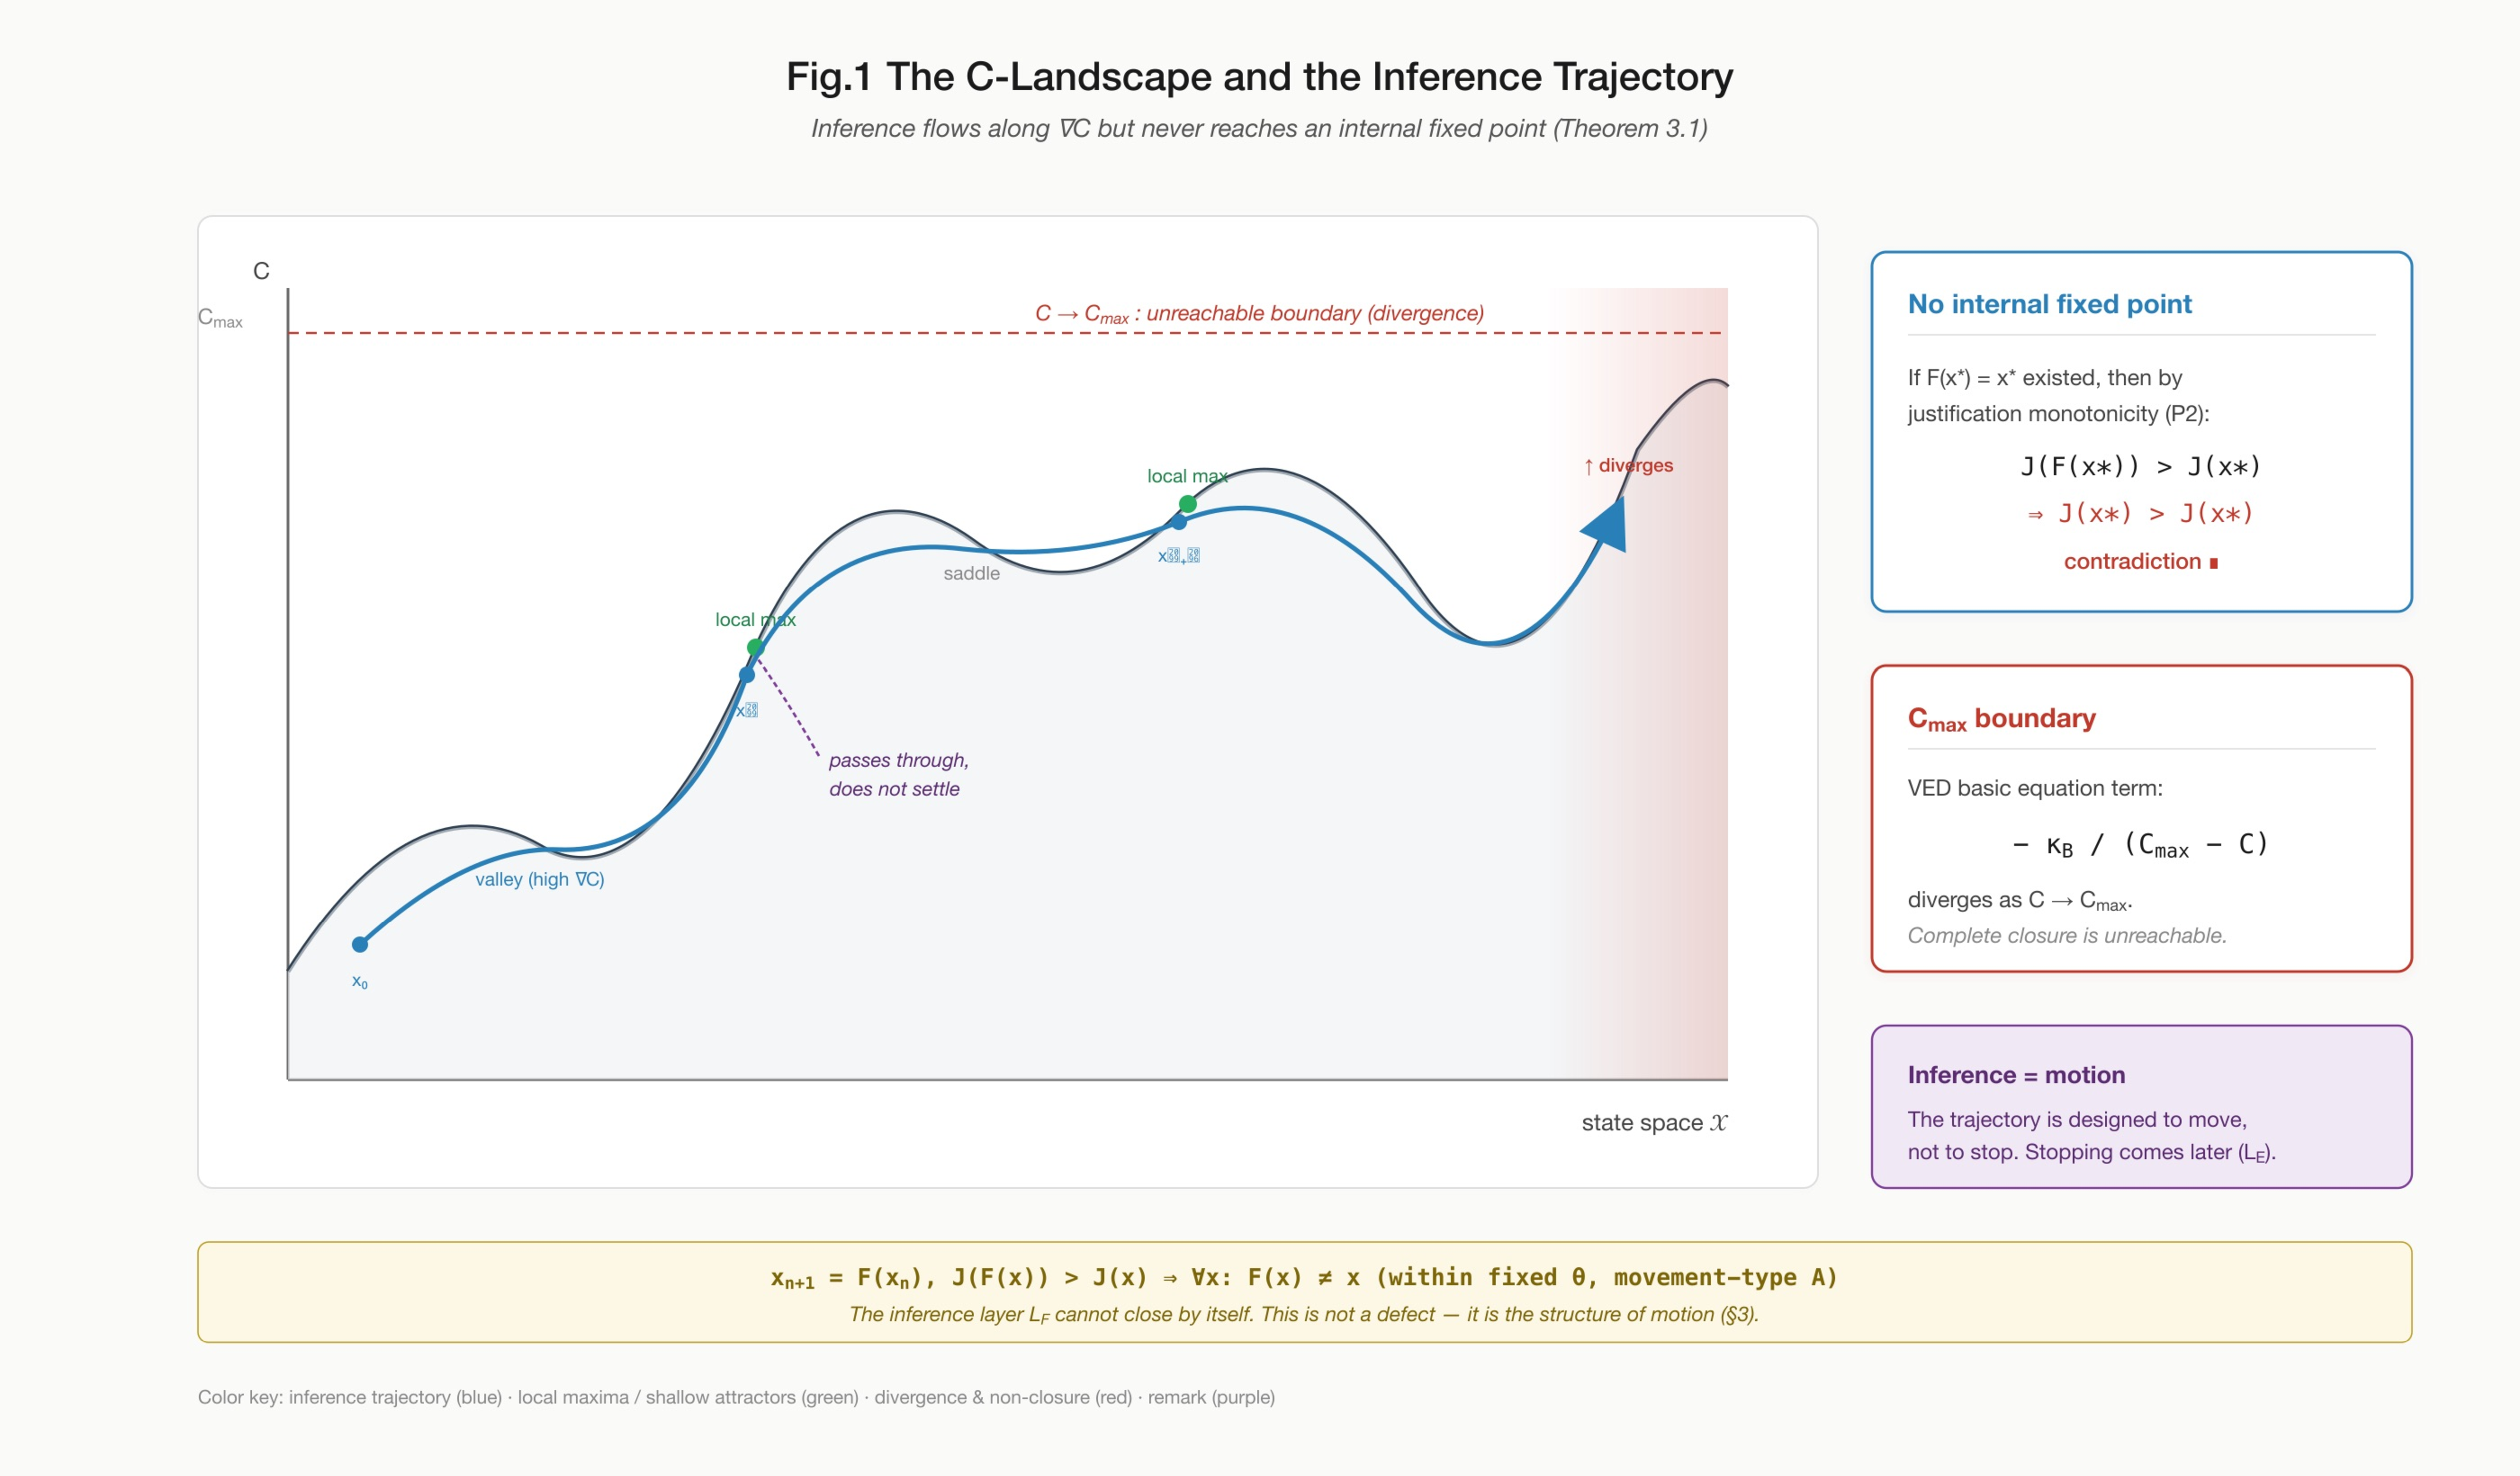
\includegraphics[width=\linewidth]{fig1_c_landscape.pdf}
\caption{The C-landscape and the inference trajectory. Inference moves along the gradient $\nabla C$ on the closure landscape, but structurally it cannot settle at an internal stopping point.}
\label{fig:part2-c-landscape}
\figurenote{The horizontal axis is state space and the vertical axis is closure degree $C$. The blue trajectory represents iterations of $F$, while the red boundary marks the unattainable $C_{\max}$.}{Within fixed $\theta$ and movement type (A), $L_F$ has no internal fixed point. The figure gives the geometric intuition for why $\mu_\theta$, region reconfiguration, and $L_E$ become necessary.}
\end{figure}

\subsection{Assumptions}

The proof requires only minimal assumptions.

\textbf{P1: Justification extension.} The inference operator $F$ sends a state $x_n$ to a more justified state $x_{n+1}=F(x_n)$.

\textbf{P2: Monotonic justification measure.} There exists a measure $J$ such that
\[
J(F(x))>J(x)
\]
for admissible states.

\textbf{P3: Fixed movement region.} The argument is made within a fixed movement region $\Omega_\theta$. It concerns movement type (A), not reconfiguration type (B).

\subsection{Theorem}

\textbf{Theorem 3.1 (Non-Closure Theorem).}
For any inference operator $F$ satisfying P1 and P2, there is no internal fixed point $x^*$ such that
\[
F(x^*)=x^*.
\]
Equivalently,
\[
\forall x\in\mathcal{X},\quad F(x)\neq x
\]
within the range of fixed-$\theta$ inference.

\subsection{Proof Sketch}

Assume, for contradiction, that a fixed point $x^*$ exists. Then $F(x^*)=x^*$. By P2,
\[
J(F(x^*))>J(x^*).
\]
But since $F(x^*)=x^*$, this becomes
\[
J(x^*)>J(x^*),
\]
which is impossible. Therefore no such internal fixed point exists.

The proof is short because the result follows from the minimal meaning of inference as justification extension. Once inference is defined as an operation that advances justification, an internal stopping point is structurally excluded.

\subsection{Branching Explosion}

The absence of an internal fixed point has two dynamical faces. First, the trajectory does not become still. Second, when inference has probabilistic or generative structure, the trajectory is not single. It branches.

This is the branching explosion introduced in Part I. In the present context it is re-described as the inability of an internal stopping condition to stop branching. The increase of inferential capacity may therefore accelerate branching explosion rather than suppress it. The problem of intelligence shifts from strengthening inference itself to operating enlarged branching in a stoppable form.

\subsection{Consequence}

The inference layer $L_F$ cannot be the whole of intelligence. If intelligence stopped nowhere, it would dissolve into regress or explosion. If it stopped by an internal predicate, that predicate would require further inference. Stopping must therefore be supplied from outside $F$ as such. \S{}5 explains how this occurs through $L_R$ and $L_E$.

\bigskip

% English draft based on sections/04_response_channels_ja.tex
\section{Response Channels and Silent Worlds}

\S{}3 showed that $L_F$ has no internal stopping condition. This chapter asks how that non-closure appears in different operating environments. The distinction between responsive and silent worlds is not ontological. It is a threshold phenomenon.

\subsection{Responsive and Silent Regimes}

A responsive world is an environment in which an inferential output receives a return. The agent asks, acts, hypothesizes, or experiments, and the world responds. In C-geometry, the gradient forms a closed loop: the output changes the world, and the changed world returns as feedback.

A silent world is an environment in which such return does not close. The agent can output inference, but no corresponding response comes back. Ultimate reasons, fixed past events, and unresolved future contingencies often appear in this mode.

Formally, a responsive regime has significant mutual constraint in both directions, $H_{ij}$ and $H_{ji}$. A silent regime has a broken or negligible return channel, approximately $H_{ji}\approx 0$.

\subsection{Silence Is Not Defect}

Silence is not a defect in the world. It is not merely ignorance waiting to be solved. Some regions do not return the kind of response required to close the inferential loop. If responsive-world strategies are applied to silent-world regions without threshold mobility, inference can enter infinite regress.

\subsection{Threshold Phenomenon}

Responsive and silent regimes are phases determined by thresholds. The same environment can appear responsive or silent depending on the position of the boundary set by parameters such as inferential velocity, resolution, and stopping hardness. The threshold mobility $\mu_\theta$ is the ability to move this boundary.

\begin{figure}[H]
\centering
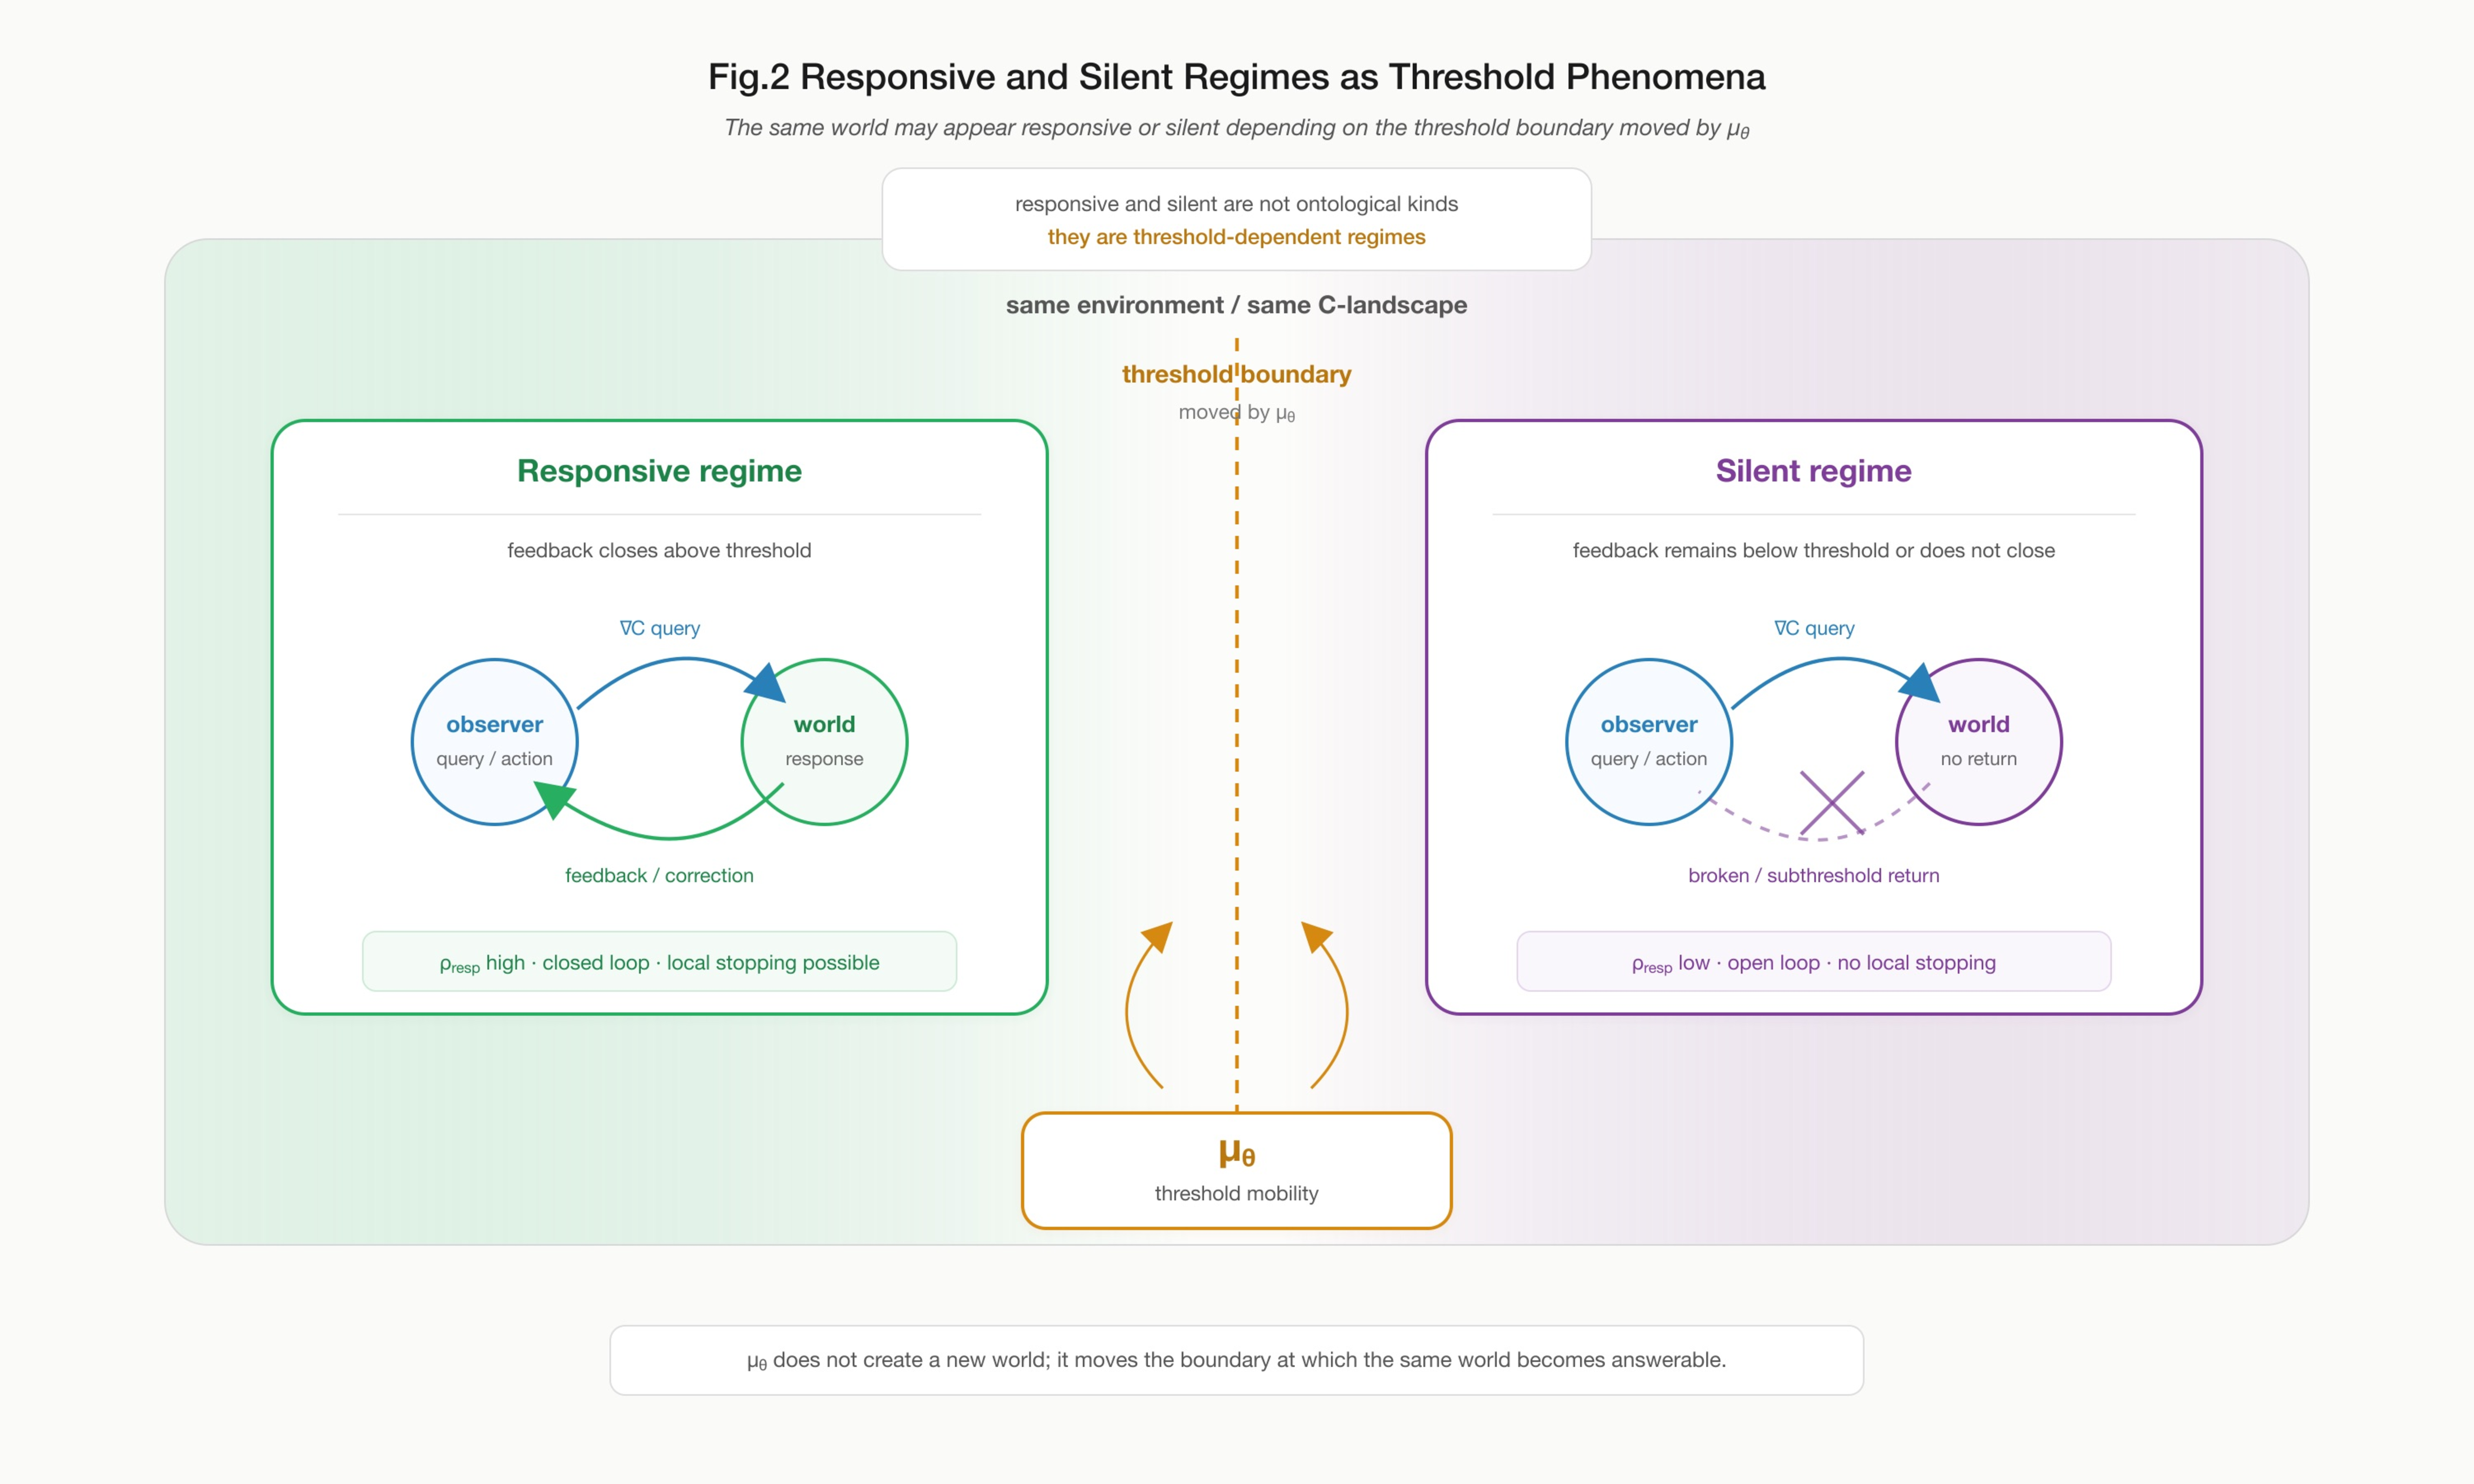
\includegraphics[width=\linewidth]{fig2_responsive_silent_threshold.pdf}
\caption{Responsive and silent regimes. These are not two ontological kinds of world, but threshold-dependent phases determined by the boundary moved by $\mu_\theta$.}
\label{fig:part2-responsive-silent}
\figurenote{Both panels share the same environment and the same C-landscape. What changes is the threshold boundary that determines whether a response loop closes.}{In the responsive phase, external mutual constraint supplies local stopping. In the silent phase, this supply is cut off, creating pressure to externalize stopping elsewhere.}
\end{figure}

\subsection{Infinite Regress in Silent Worlds}

If an agent is fixed in a silent regime, three conditions hold: the environment does not return a stopping response, justification can only be advanced by inference, and stopping cannot be derived from inference itself. Under these conditions, inference lacks a stopping resource and continues indefinitely.

Infinite regress and branching explosion are two aspects of the same structural fact. Internal non-fixedness means the trajectory does not become still; branching means the trajectory is not single. In silent regimes, the two combine. The result is a doubly unstable dynamics.

\subsection{The Preview of $L_R$}

Non-stopping inference leaves traces. The trajectory records where it passed, which branches it attempted, and where it diverged. These traces form logs. Recursive reference to such logs is the beginning of the log layer $L_R$.

This is the bridge to \S{}5. The failure of $L_F$ to stop is not only a dead end. It is also productive: because inference does not stop, traces accumulate; because traces accumulate, recursive reference becomes possible; because recursive reference becomes possible, $L_E$ can emerge under external mutual constraint.

\bigskip

% English draft based on sections/05_emergent_stopping_layer_ja.tex
\section{The Emergent Stopping Layer $L_E$}

This chapter is the second center of the paper. \S{}3 showed that $L_F$ does not close by itself. This chapter shows how intelligence nevertheless stops: through the log layer $L_R$ and the emergent stopping layer $L_E$.

\begin{figure}[H]
\centering
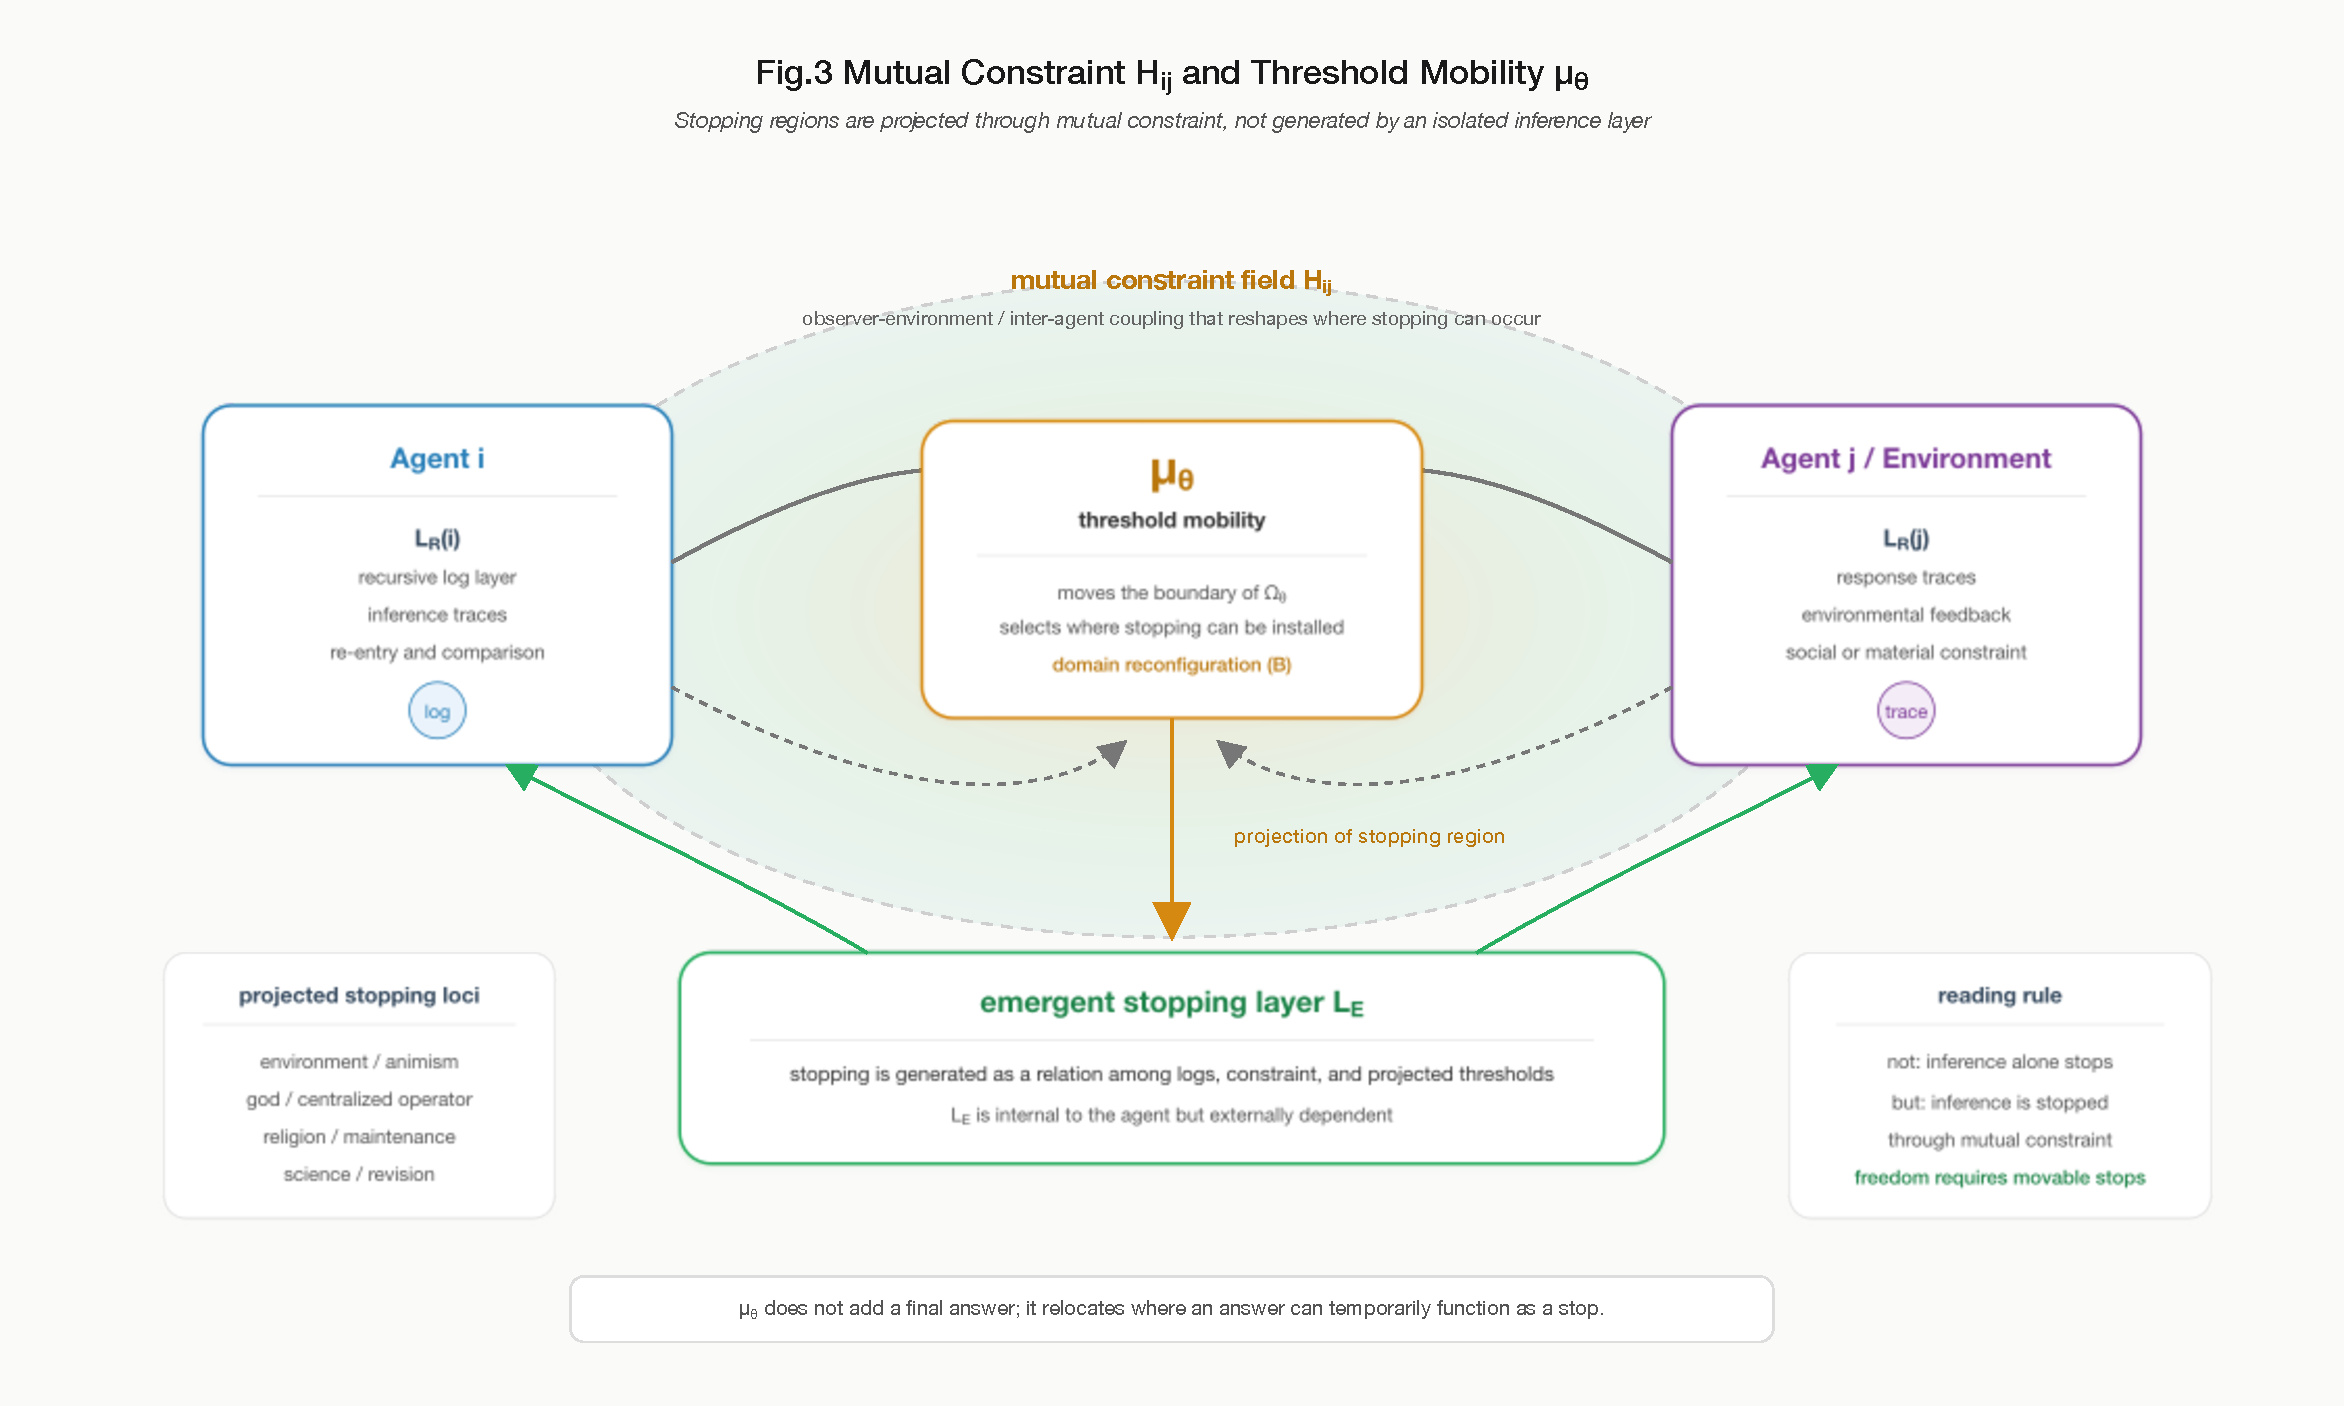
\includegraphics[width=\linewidth]{fig3_mutual_constraint_mu_theta.pdf}
\caption{Mutual constraint $H_{ij}$ and threshold mobility $\mu_\theta$. Stopping regions are not generated by an isolated inference layer; they are projected through mutual constraint.}
\label{fig:part2-mutual-constraint}
\figurenote{$H_{ij}$ changes where stopping can occur. $\mu_\theta$ reorganizes the possible installation region of the stopping operator $E$.}{Stopping is not found inside $L_F$. It is projected and emerges as $L_E$ from the relation between $L_R$ and $H_{ij}$. Movable stopping is a condition of sustained freedom.}
\end{figure}

\begin{figure}[H]
\centering
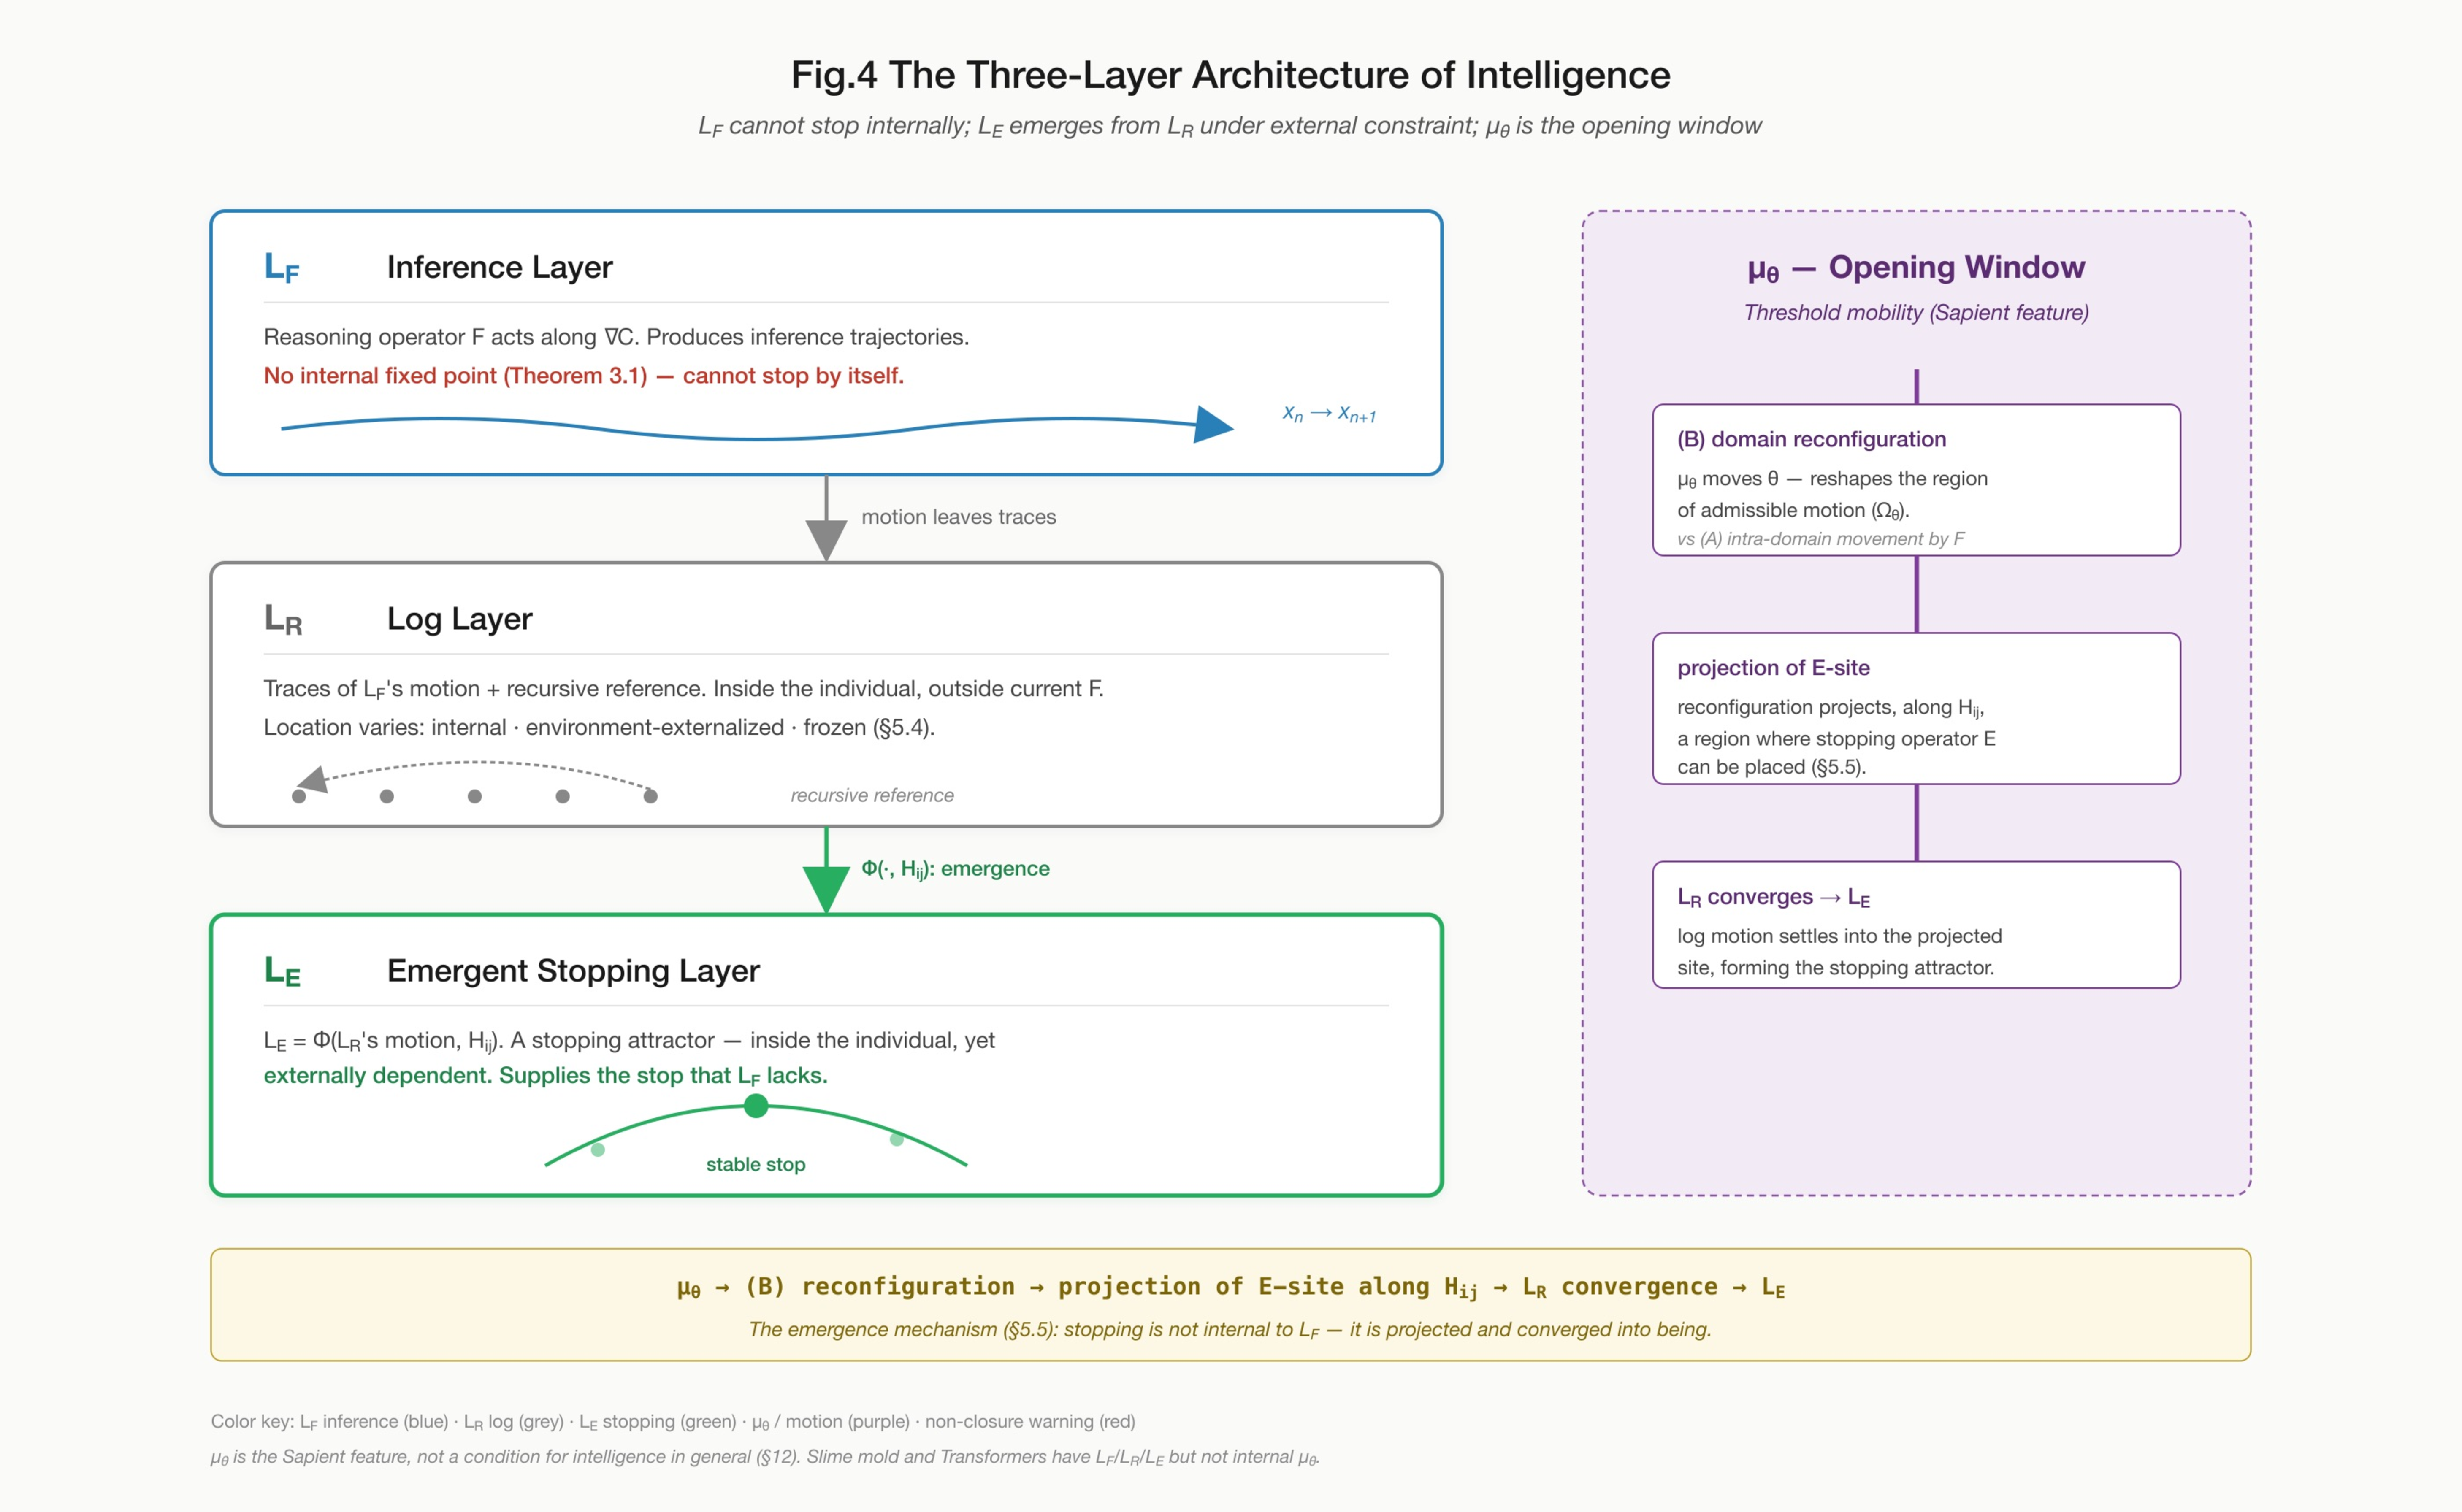
\includegraphics[width=\linewidth]{fig4_three_layer_architecture.pdf}
\caption{The three-layer architecture of intelligence. Intelligence consists of $L_F$, $L_R$, and $L_E$; $\mu_\theta$ is the opening window through which stopping regions can be reconfigured.}
\label{fig:part2-three-layer}
\figurenote{$L_F$ cannot stop by itself. Its motion leaves traces in $L_R$, and recursive log motion under $H_{ij}$ gives rise to $L_E$.}{The figure joins the two centers of the paper: non-closure in \S{}3 and emergent stopping in \S{}5. The limit of $L_F$ becomes the condition for higher-layer formation.}
\end{figure}

\subsection{Problem Setting}

Real intelligence stops. Humans end a chain of reasoning, make judgments, and act. Since \S{}3 showed that stopping does not come from inside $L_F$, it must come from elsewhere. The question is what ``elsewhere'' means.

The answer is that stopping comes from a layer that is internal to the individual but externally dependent: the emergent stopping layer $L_E$.

\subsection{The Log Layer $L_R$}

The log layer $L_R$ is the layer of recursive reference to traces left by inference. These traces include passed states, attempted branches, failed paths, and points of divergence. $L_R$ is inside the individual in many systems, but outside the current operation of $F$.

The location of $L_R$ differs by system. In a slime mold, logs can be externalized into the environment as slime traces. In a Transformer, training data are frozen logs and context tokens are volatile logs. In sapiens-like intelligence, logs exist both individually and socially.

\subsection{Definition of $L_E$}

\textbf{Definition 5.1 (Emergent stopping layer).}
The emergent stopping layer $L_E$ is a stopping layer that dynamically emerges as a function of the recursive motion of $L_R$ and external mutual constraint $H_{ij}$:
\[
L_E=\Phi(L_R\text{ motion},H_{ij}).
\]
It is internal to the agent but externally dependent.

\begin{figure}[H]
\centering
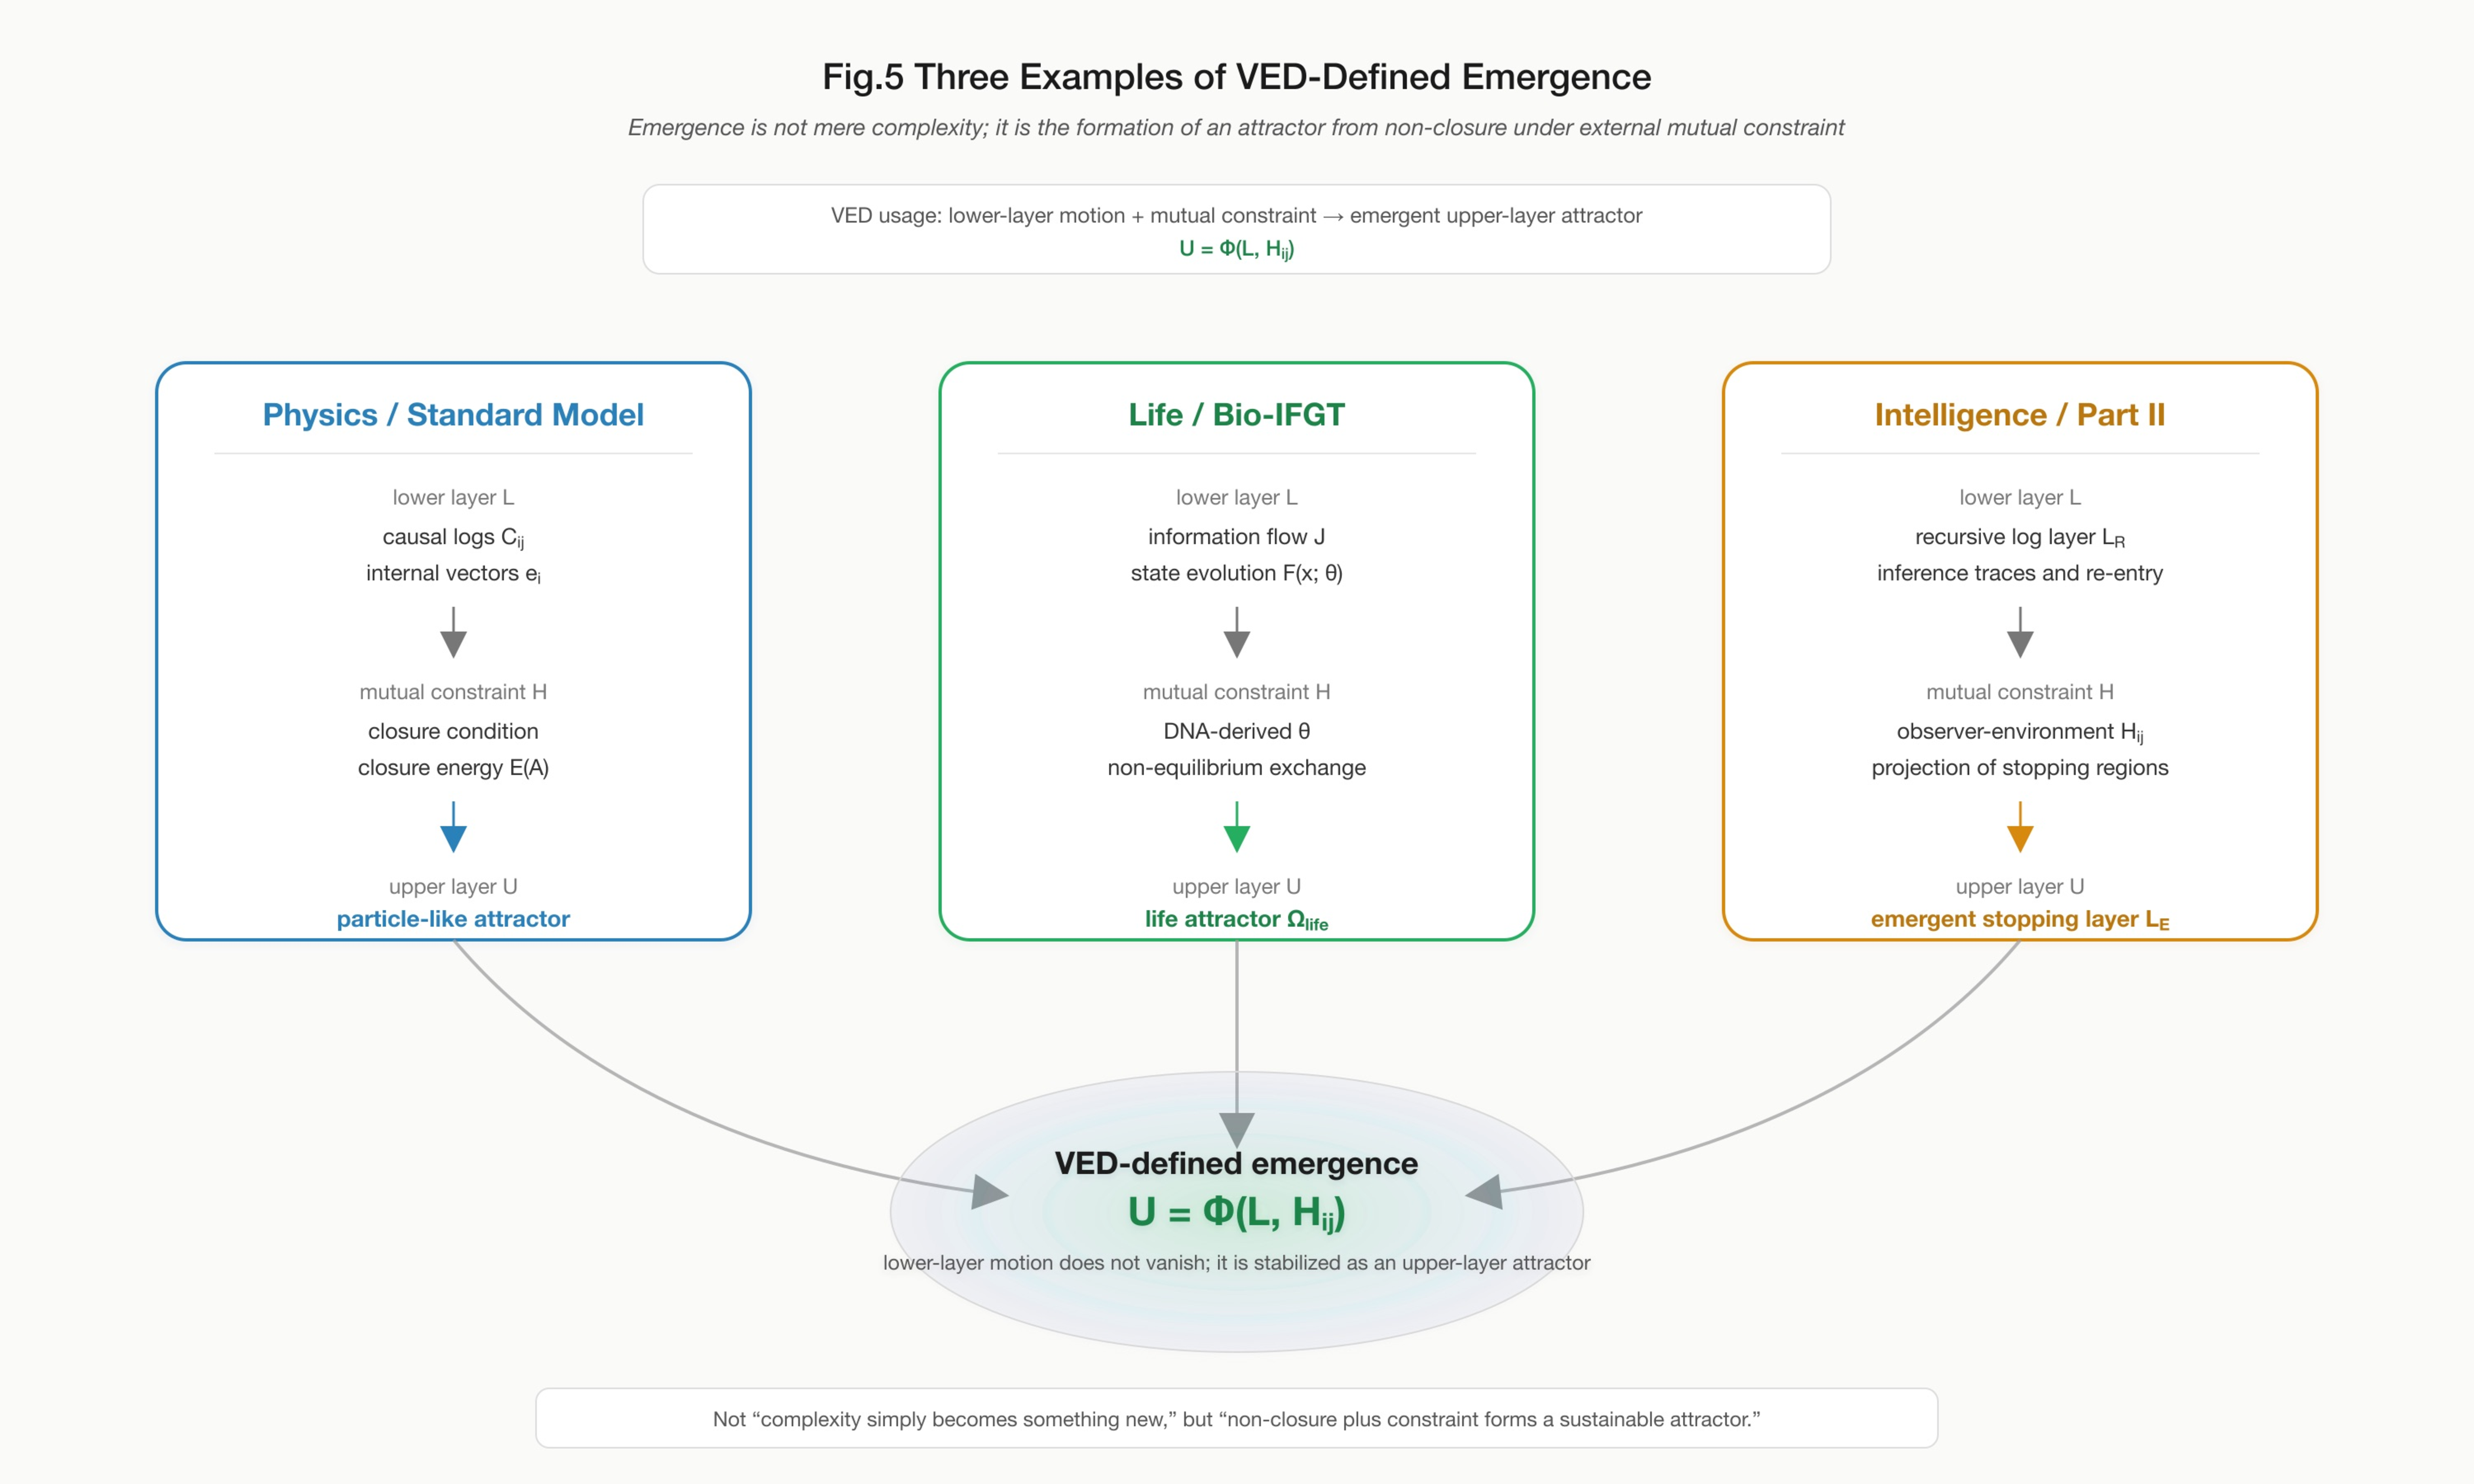
\includegraphics[width=\linewidth]{fig5_three_examples_of_emergence.pdf}
\caption{Three examples of VED-defined emergence. Emergence is the formation of an upper attractor from lower non-closed motion under external mutual constraint $H_{ij}$.}
\label{fig:part2-emergence-examples}
\figurenote{Particle attractors, the life attractor $\Omega_{\text{life}}$, and the stopping layer $L_E$ can all be read as substitutions into $U=\Phi(L,H_{ij})$.}{Emergence is not mere complexity. It is the stabilization of non-closed motion as an attractor under mutual constraint, linking $L_E$ to the broader VED theory tree.}
\end{figure}

\subsection{Three Profiles}

Three systems clarify the variability of $L_R$, $\mu_\theta$, and $L_E$.

\textbf{Slime mold.} Its logs are environmental; its stopping is generated by direct environmental interaction; its $\mu_\theta$ is largely fixed.

\textbf{Transformer.} Its logs are internalized as frozen weights and volatile context; its stopping is externally injected through EOS tokens, task specifications, or decoding controls; it does not generate its own $L_E$ in the sense used here.

\textbf{Sapiens.} Logs are both individual and social; $L_E$ emerges internally and is socially synchronized; $\mu_\theta$ can be moved endogenously.

\subsection{Emergence Mechanism}

The emergence of $L_E$ proceeds in four stages:
\begin{enumerate}
\item $\mu_\theta$ causes region reconfiguration (B);
\item the reconfiguration projects a possible installation region for the stopping operator $E$;
\item the recursive motion of $L_R$ converges into the projected region;
\item the resulting stable stopping attractor is $L_E$.
\end{enumerate}

Schematically:
\[
\mu_\theta \to (B)\text{ reconfiguration} \to E\text{-region projection} \to L_R\text{ convergence} \to L_E .
\]

This mechanism shows that stopping is not the negation of freedom. Without projected stopping regions, inference becomes unsustainable in branching explosion and infinite regress. $L_E$ emerges not to restrict freedom, but to make free inference sustainable within a finite system.

\subsection{Projection}

The projection used here is the intelligence-layer realization of the projection primitive fixed in the consciousness paper. It means that a state or relation acquires unequal influence within a field. In this paper, the projected object is a possible stopping locus.

\subsection{External Stopping Operator}

The external stopping operator $E$ is the action of $L_E$ on an inferential state:
\[
E=E[L_E,x_n],\qquad E\notin\{F^k\}.
\]
It is external because it is not a member of the sequence of inference operations. It acts through $L_E$.

\subsection{$\Phi_{\text{ext}}\equiv\Phi_{\text{net}}$}

The external reference field $\Phi_{\text{ext}}$ is isomorphic to the inter-individual network of emergent stopping layers $\Phi_{\text{net}}$:
\[
\Phi_{\text{ext}}\equiv\Phi_{\text{net}}.
\]
Here $\Phi_{\text{ext}}$ should be read as an intelligence-layer projection of the IFGT potential vocabulary, not as the full IFGT field itself. It names the way a shared stopping structure appears as an external reference field from within an individual inference window.

\begin{figure}[H]
\centering
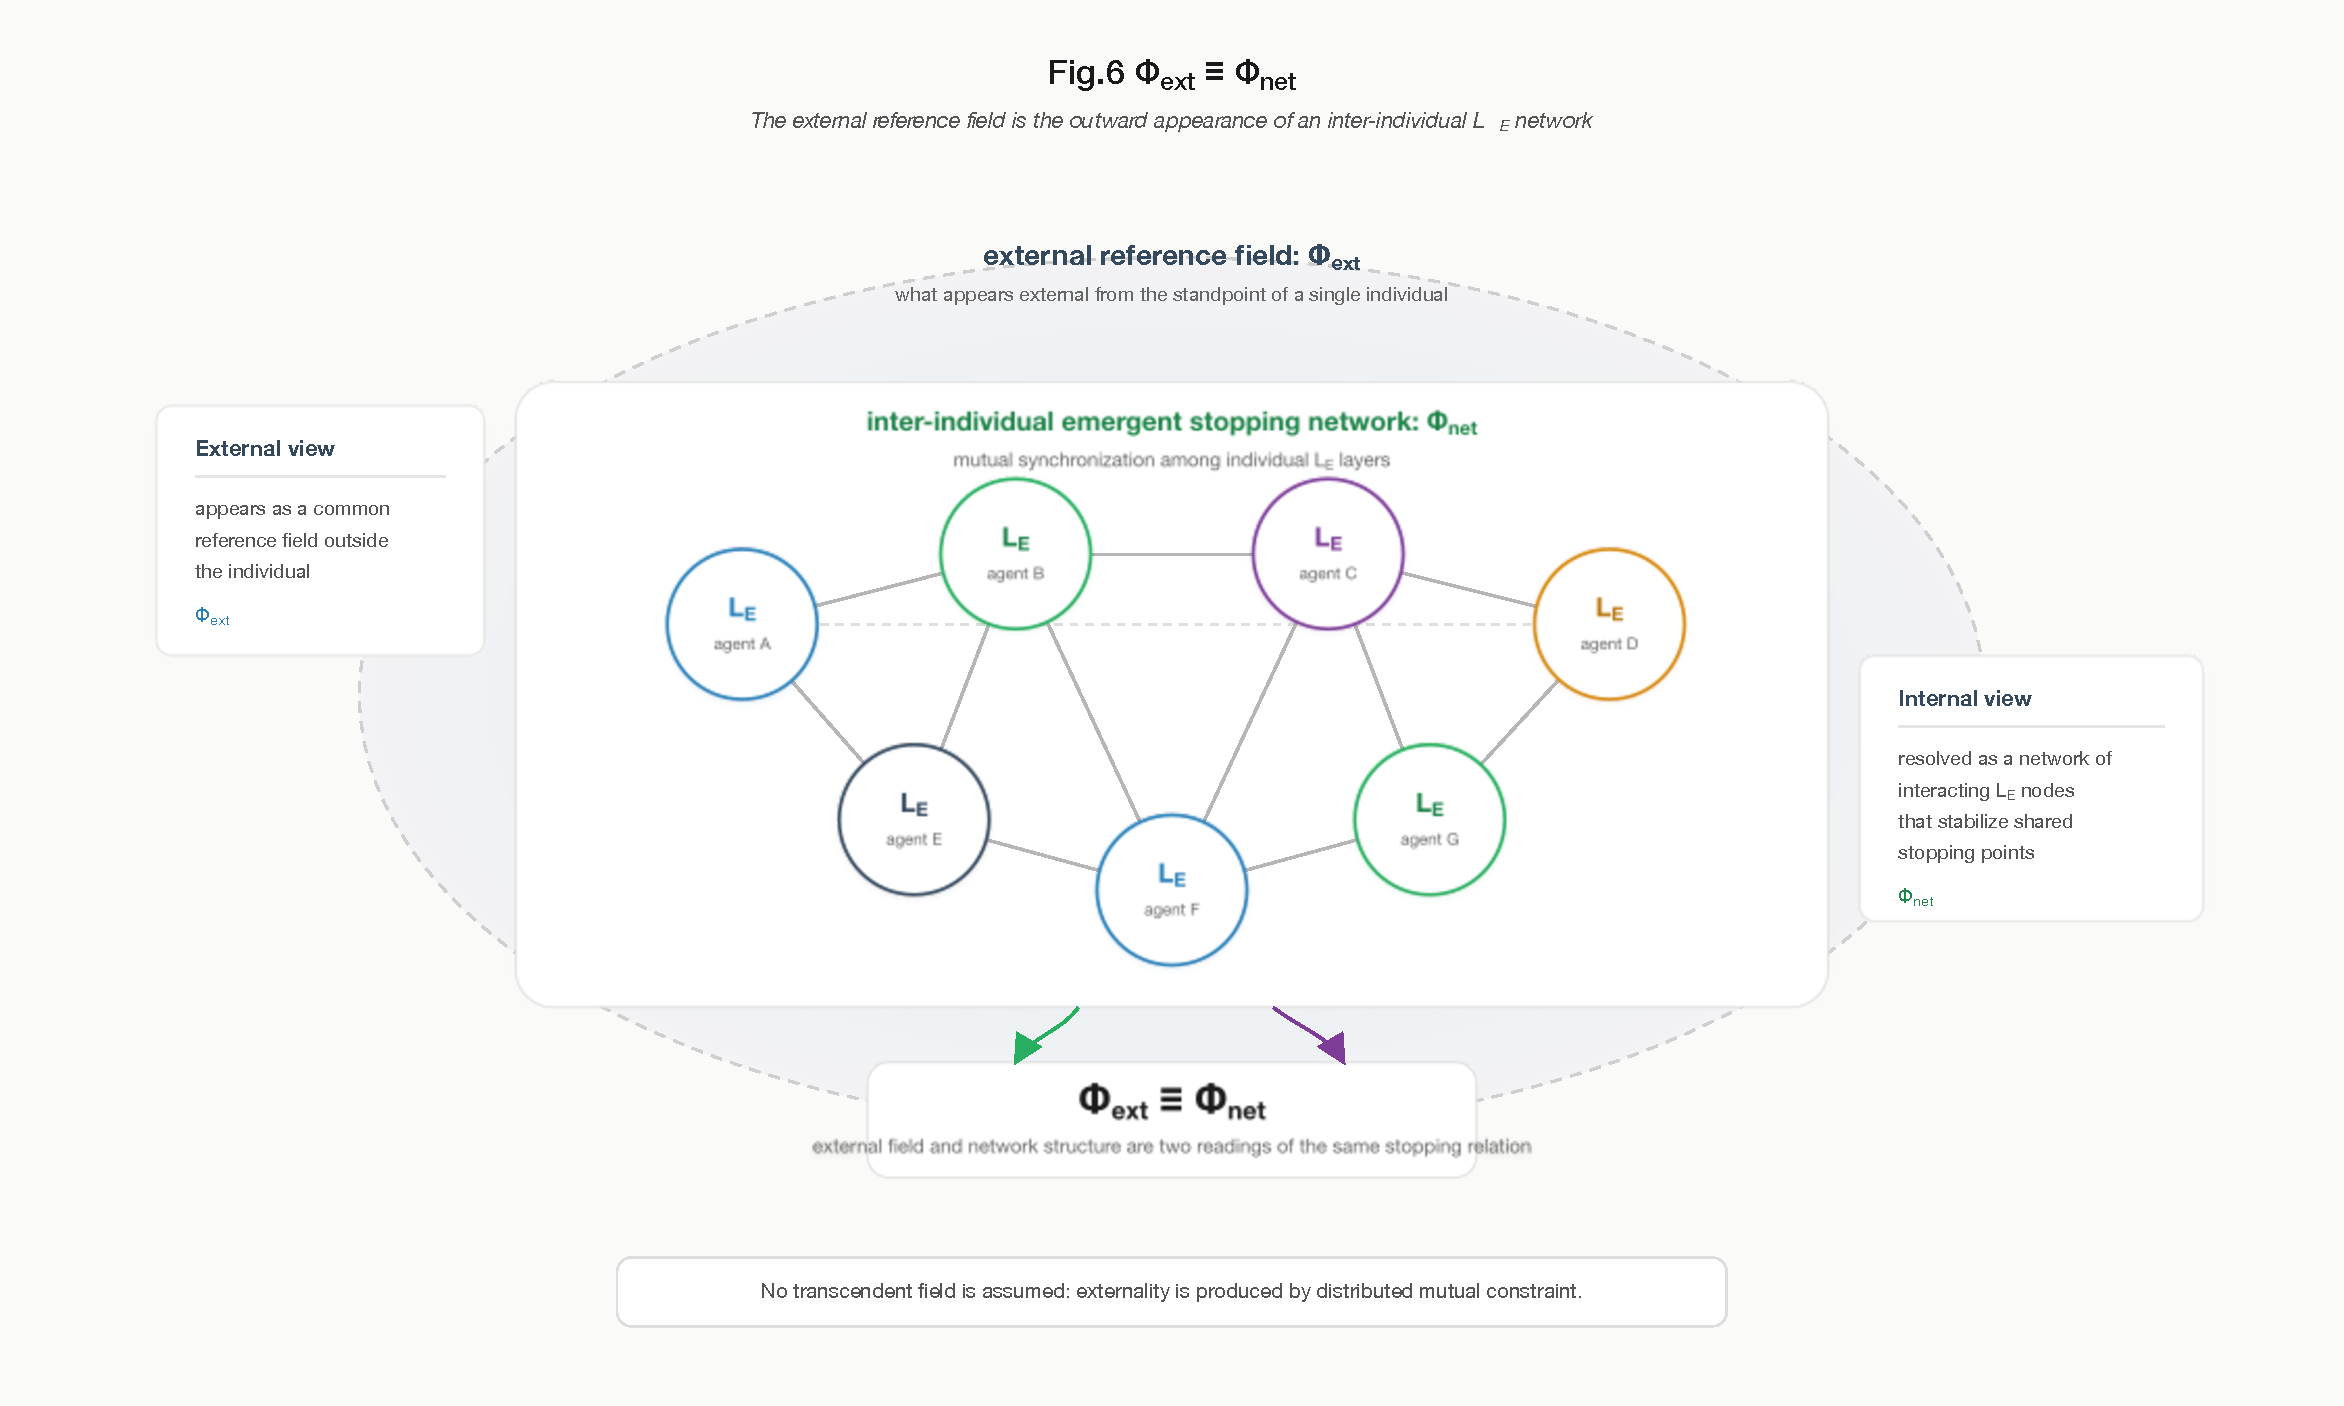
\includegraphics[width=\linewidth]{fig6_phi_ext_phi_net.pdf}
\caption{$\Phi_{\text{ext}} \equiv \Phi_{\text{net}}$. What appears to an individual as an external reference field is the network formed by mutual synchronization among individual $L_E$ layers.}
\label{fig:part2-phi-ext-net}
\figurenote{$\Phi_{\text{ext}}$ is the external appearance; $\Phi_{\text{net}}$ is the internal network structure of mutually synchronized $L_E$ layers.}{No transcendent field needs to be assumed. Norms, gods, truth, and monetary value can be read as appearances of distributed $L_E$ synchronization.}
\end{figure}

\subsection{Summary}

Intelligence persists through the simultaneous motion of $L_F$, $L_R$, and $L_E$ under externally dependent stopping. Sapiens-like intelligence adds endogenous $\mu_\theta$, allowing stopping loci to be reorganized rather than merely received.

\bigskip

% English draft based on sections/06_animism_ja.tex
\section{Animism: Installation of Stopping in the Environment}

Animism is treated here not as an error about spirits, but as an early operating form of stopping structures. It installs stopping loci in the environment.

In silent or under-responsive regions, inference cannot obtain sufficient return from the world. Animistic operation assigns stopping power to places, objects, winds, stones, rivers, animals, or events. Structurally, this means that an external element is made into a locus at which inference may stop, orient, or act.

This does not require the theory to assert the existence of spirits. Nor does it require the theory to dismiss animism as illusion. The question is structural: what operation does animism perform for finite intelligence? Its answer is that animism distributes $L_E$ into the environment.

This form is close to environmental mutual constraint. The stopping locus is not yet centralized. It is local, concrete, and embedded in direct interaction between agent and environment. In this sense, animism is an installation operation:
\[
\text{environmental locus} \;\mapsto\; E\text{-installation site}.
\]

The importance of animism in this theory is that it shows stopping before centralization. The environment itself is used as a distributed surface on which stopping can be projected.

\bigskip

% English draft based on sections/07_god_ja.tex
\section{God: Compression of Distributed Stopping}

If animism distributes stopping across many environmental loci, the figure of God compresses stopping into a central reference point. The function analyzed here is not theological proof or disproof, but structural compression.

Distributed stopping is flexible but ambiguous. Many loci can conflict. A centralized stopping point reduces ambiguity by gathering multiple stopping functions into one high-weight reference. In the language of this paper, God is a compressed $\Phi_{\text{ext}}$.

This does not make God the historical endpoint of a progress narrative. God is treated here as a structural pole of compression: one possible operation by which distributed stopping is gathered, weighted, and stabilized.

This compression has stabilizing power. It provides a unified answer to questions that otherwise remain silent. It can close regress, coordinate communities, and bind action to a common orientation.

Yet compression also carries risk. If the compressed stopping point becomes too rigid, it can produce hard closure. The problem is not that stopping exists, but that stopping loses revisability. The later distinction between religion, science, and social blockchain can be read as different responses to this risk.

God is therefore positioned as an operation in the history of stopping structures:
\[
\text{distributed stopping} \;\longrightarrow\; \text{centralized stopping}.
\]

\bigskip

% English draft based on sections/08_religion_ja.tex
\section{Religion: Long-Term Maintenance of Stopping Structures}

Religion is treated here as a large-scale system for the long-term maintenance of stopping structures. It stabilizes stopping across time, generations, communities, rituals, texts, and institutions.

The problem religion solves is not merely belief. It is durability. A stopping point that exists only in one individual disappears with that individual. A stopping point that is ritually repeated, textually preserved, socially enforced, and institutionally transmitted becomes durable.

In the vocabulary of this paper, religion maintains $L_E$ across generations. It keeps stopping structures available in regions where inference alone would reopen regress.

This maintenance can be constructive. It protects finite intelligence from dissolution into endless questioning. It can preserve shared orientation, responsibility, and collective memory. But it can also harden. If the stopping structure loses revisability, religion can enter rigid attractors: absolutism, private closure, or refusal of new response.

The structural point is value-neutral. Religion is neither reduced to error nor elevated above critique. It is an operating form of stopping maintenance:
\[
\text{centralized stopping} \;\longrightarrow\; \text{maintained stopping}.
\]

This prepares the role of science. If religion strongly maintains stopping, science institutionalizes the revision of stopping.

\bigskip

% English draft based on sections/09_social_blockchain_ja.tex
\section{Social Blockchain: Distributed $L_E$ as $\Phi_{\text{net}}$}

\S{}6--\S{}8 described environmental installation, central compression, and long-term maintenance of stopping. This chapter describes a form that maintains stopping without reducing it to a single authority: distributed social stopping. This is called social blockchain.

The term is structural. It does not refer to cryptocurrency or to a specific distributed-ledger implementation. What is borrowed is only the structural feature: distributed nodes form provisional consensus without a single central authority, while keeping the consensus revisable.

\subsection{Structure}

The central feature of social blockchain is the coexistence of stopping and updating without a single authority. Individual nodes generate provisional stops. Logs preserve the history of judgments and their grounds. Forks represent divergent stopping candidates. Merges and abandonments reorganize stopping.

Unlike technical version control, social blockchain is not optimized for free branching. Branching can be costly because it can mean social division. Merging is slow because consensus takes time. Rollback is difficult because accepted stopping points carry responsibility and history.

The center is therefore not Version Control but Consensus.

\subsection{Legitimacy Rather Than Consistency}

Technical blockchains address consistency: can distributed nodes agree on a non-contradictory state? Social blockchain addresses legitimacy: can a distributed stopping point be accepted as legitimate?

Legitimacy is not computable in the same sense. It depends on time, responsibility, historical acceptance, and distributed recognition. This non-computability is not a defect. It is the reason social stopping can remain revisable instead of being frozen by an algorithm.

\subsection{Creation and Stabilization}

Creation occurs in individual nodes. Society stabilizes after the fact. A new concept, hypothesis, or dimension arises when an individual $L_F$ reaches the boundary of an existing quasi-closure. This is unstable. The social network then accepts, rejects, records, revises, or synchronizes the result.

Individual nodes create; $\Phi_{\text{net}}$ stabilizes. One cannot replace the other.

\subsection{Position in the Three-Layer Dynamics}

Social blockchain is a form of $\Phi_{\text{net}}$: the explicit distributed operation of inter-individual $L_E$ networks.

\S{}6--\S{}8 can now be positioned as a sequence. Animism distributes $L_E$ into the environment. God centralizes $L_E$. Religion maintains centralized $L_E$ across generations. Social blockchain operates the $L_E$ network itself without centralizing it.

\begin{figure}[H]
\centering
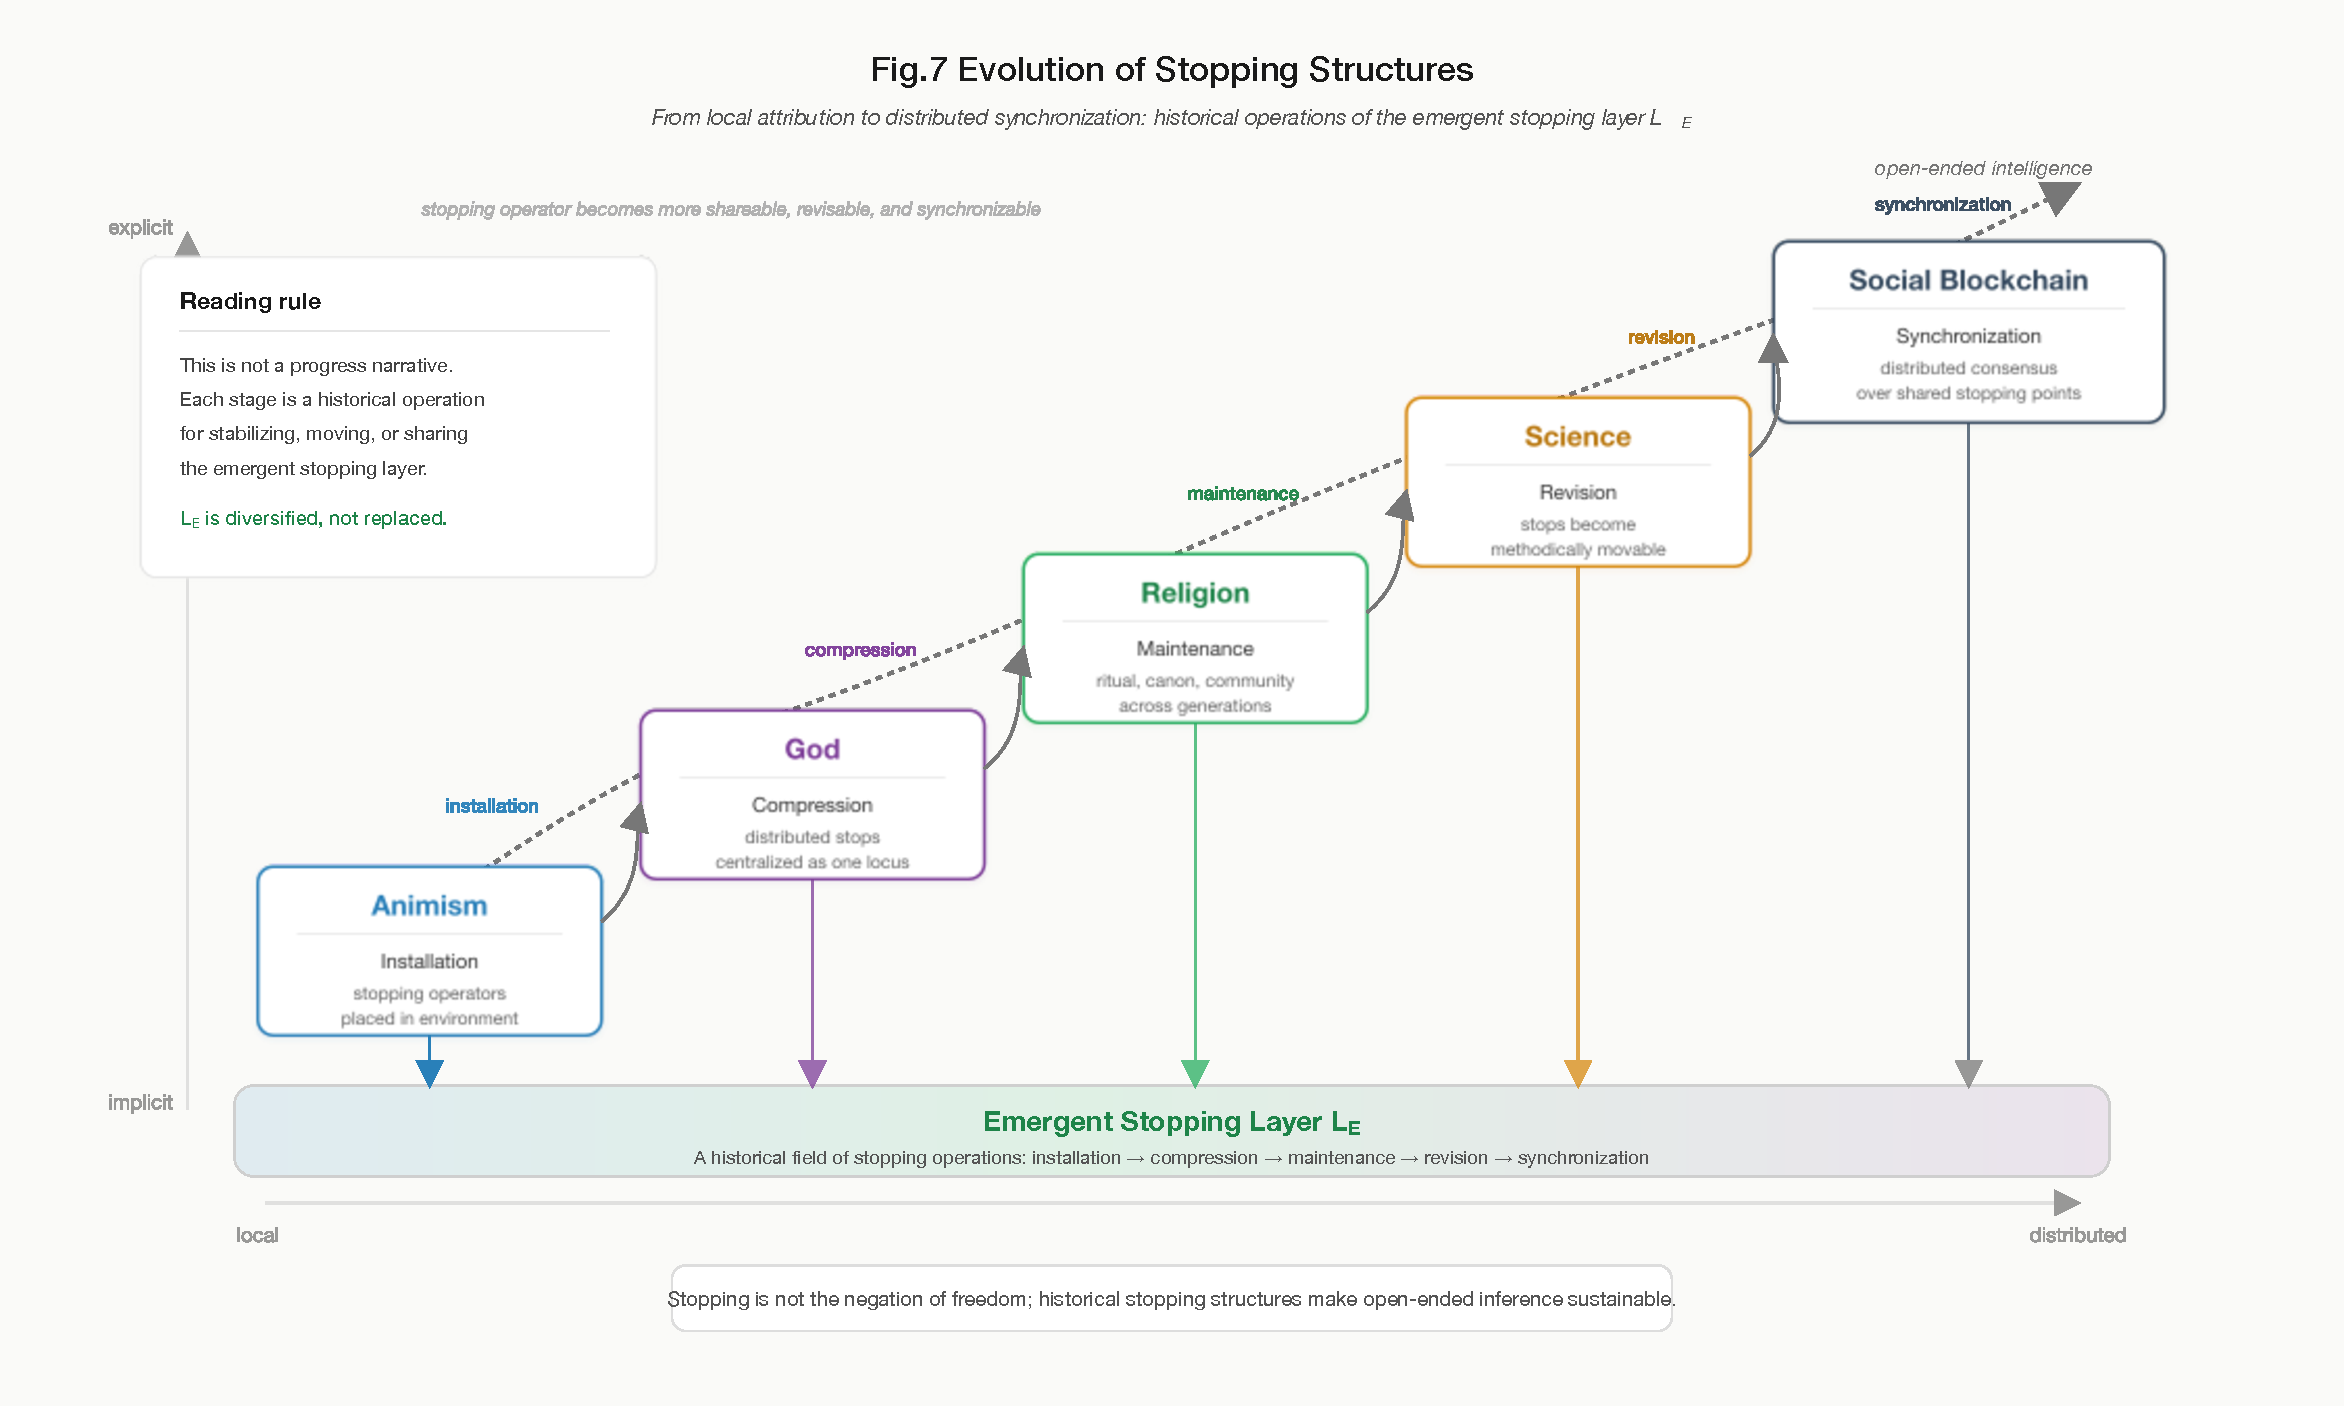
\includegraphics[width=\linewidth]{fig7_evolution_of_stopping_structures.pdf}
\caption{Evolution of stopping structures. Animism, God, religion, science, and social blockchain are different operations for stabilizing, moving, revising, and synchronizing the same emergent stopping layer $L_E$.}
\label{fig:part2-stopping-evolution}
\figurenote{The five forms are installation, compression, maintenance, revision, and synchronization. This is not a progress story, but a diversification of $L_E$ operations.}{Stopping is not the negation of freedom. Historical stopping structures are operating forms that make open-ended inference sustainable within finite systems.}
\end{figure}

If religion institutionalizes the long-term maintenance of stopping structures, science can be understood as the operating form that institutionalizes their revision. Social blockchain is then positioned above this as a mechanism for distributed sharing and synchronization of stopping structures.

\subsection{Bridge to the Gettier Problem}

In social blockchain, stopping is not guaranteed by truth. It is established through distributed acceptance and structural stability. This raises the next question: if social stopping does not guarantee truth, what is knowledge? The Gettier problem is treated in \S{}10 as a structural diagnosis of this gap.

\bigskip

% English draft based on sections/10_gettier_problem_ja.tex
\section{The Gettier Problem: Stability Is Not Truth}

The Gettier problem shows that justified true belief can still fail to be knowledge. In the present framework, this is not an anomaly in epistemology. It is evidence that closure degree $C$ is not a truth measure.

\subsection{Structural Diagnosis}

A belief can be justified, true, and yet accidentally true. Its stopping structure is stable enough to be accepted, but the path by which it arrived at truth is not structurally appropriate. The problem is therefore not simply missing justification. It is the non-identity of stability and truth.

In this paper, $L_E$ supplies revisable stopping, not guaranteed truth. A stopping point can be operationally stable while still requiring later correction. This is precisely why intelligence needs logs, external reference fields, and revision mechanisms.

\subsection{$C$ as Stability Measure}

Closure degree $C$ measures operable stability. It does not measure truth. If $C$ were truth, then higher closure would monotonically approach knowledge. Gettier cases show that this is false. A state can possess high closure and still fail as knowledge.

The correct reading is:
\[
C = \text{degree of operational closure/stability},
\]
not
\[
C = \text{truth}.
\]

\subsection{Error Tolerance and $\mu_\theta$}

The ability to move thresholds entails the ability to be wrong. If a system can reorganize its stopping region, it can install a stopping operator in a region that later proves inadequate. Error is not an accidental defect added to intelligence from outside. It is structurally linked to threshold mobility.

A perfectly correct intelligence would never need to move thresholds. But a system that never moves thresholds is rigid. Thus error tolerance and $\mu_\theta$ are structurally coupled.

\subsection{Consequence}

Knowledge requires more than immediate stopping. It requires revisable stopping supported by logs, external reference fields, and later correction. The Gettier problem therefore confirms the paper's central claim: intelligence persists not by reaching absolute closure, but by operating provisional stopping under conditions of possible revision.

\bigskip

% English draft based on sections/11_instability_region_ja.tex
\section{The Instability Region: A Three-Axis Phase Diagram}

This chapter integrates the three main logical lines of the paper: non-closure and external stopping, threshold mobility and sapiens-like acceleration, and the three-layer dynamics $L_F/L_R/L_E$.

\subsection{Three Axes}

The dynamical state of intelligence is described by three axes:
\begin{itemize}
\item inferential velocity $v_{\text{inf}}$;
\item resolution $r_{\text{res}}$;
\item stopping hardness $\eta$.
\end{itemize}

Higher inferential velocity means more inferential steps per unit time. Higher resolution means finer distinctions and causal decompositions. Higher stopping hardness means less revisability of stopping.

In addition to these three axes, the transition into divergence depends on the log-reference velocity $v_{LR}$. This is the rate at which the log layer $L_R$ can recursively reference traces generated by $L_F$ and incorporate them as usable patterns. The difference
\[
\Delta v_{\text{intel}} = v_{\text{inf}} - v_{LR}
\]
measures the speed gap between inference generation and log reference. When this gap grows too large, inference outruns the log layer and the basis for $L_E$ begins to break.

\subsection{Three Regions}

The phase space contains three regions.

\textbf{Stable operation region.} Inference is constrained by externalized stopping, $L_E$ remains revisable, and $\mu_\theta$ can operate.

\textbf{Divergent region.} High velocity and high resolution combine with internalized stopping. $L_F$ runs ahead, $L_R$ cannot follow, $L_E$ cannot emerge, and $\mu_\theta$ cannot open a window.

\textbf{Rigid region.} Stopping hardness is excessive. $L_E$ fixes, $\mu_\theta$ loses mobility, and the dynamic relation between $L_F$ and $L_E$ freezes.

\begin{figure}[H]
\centering
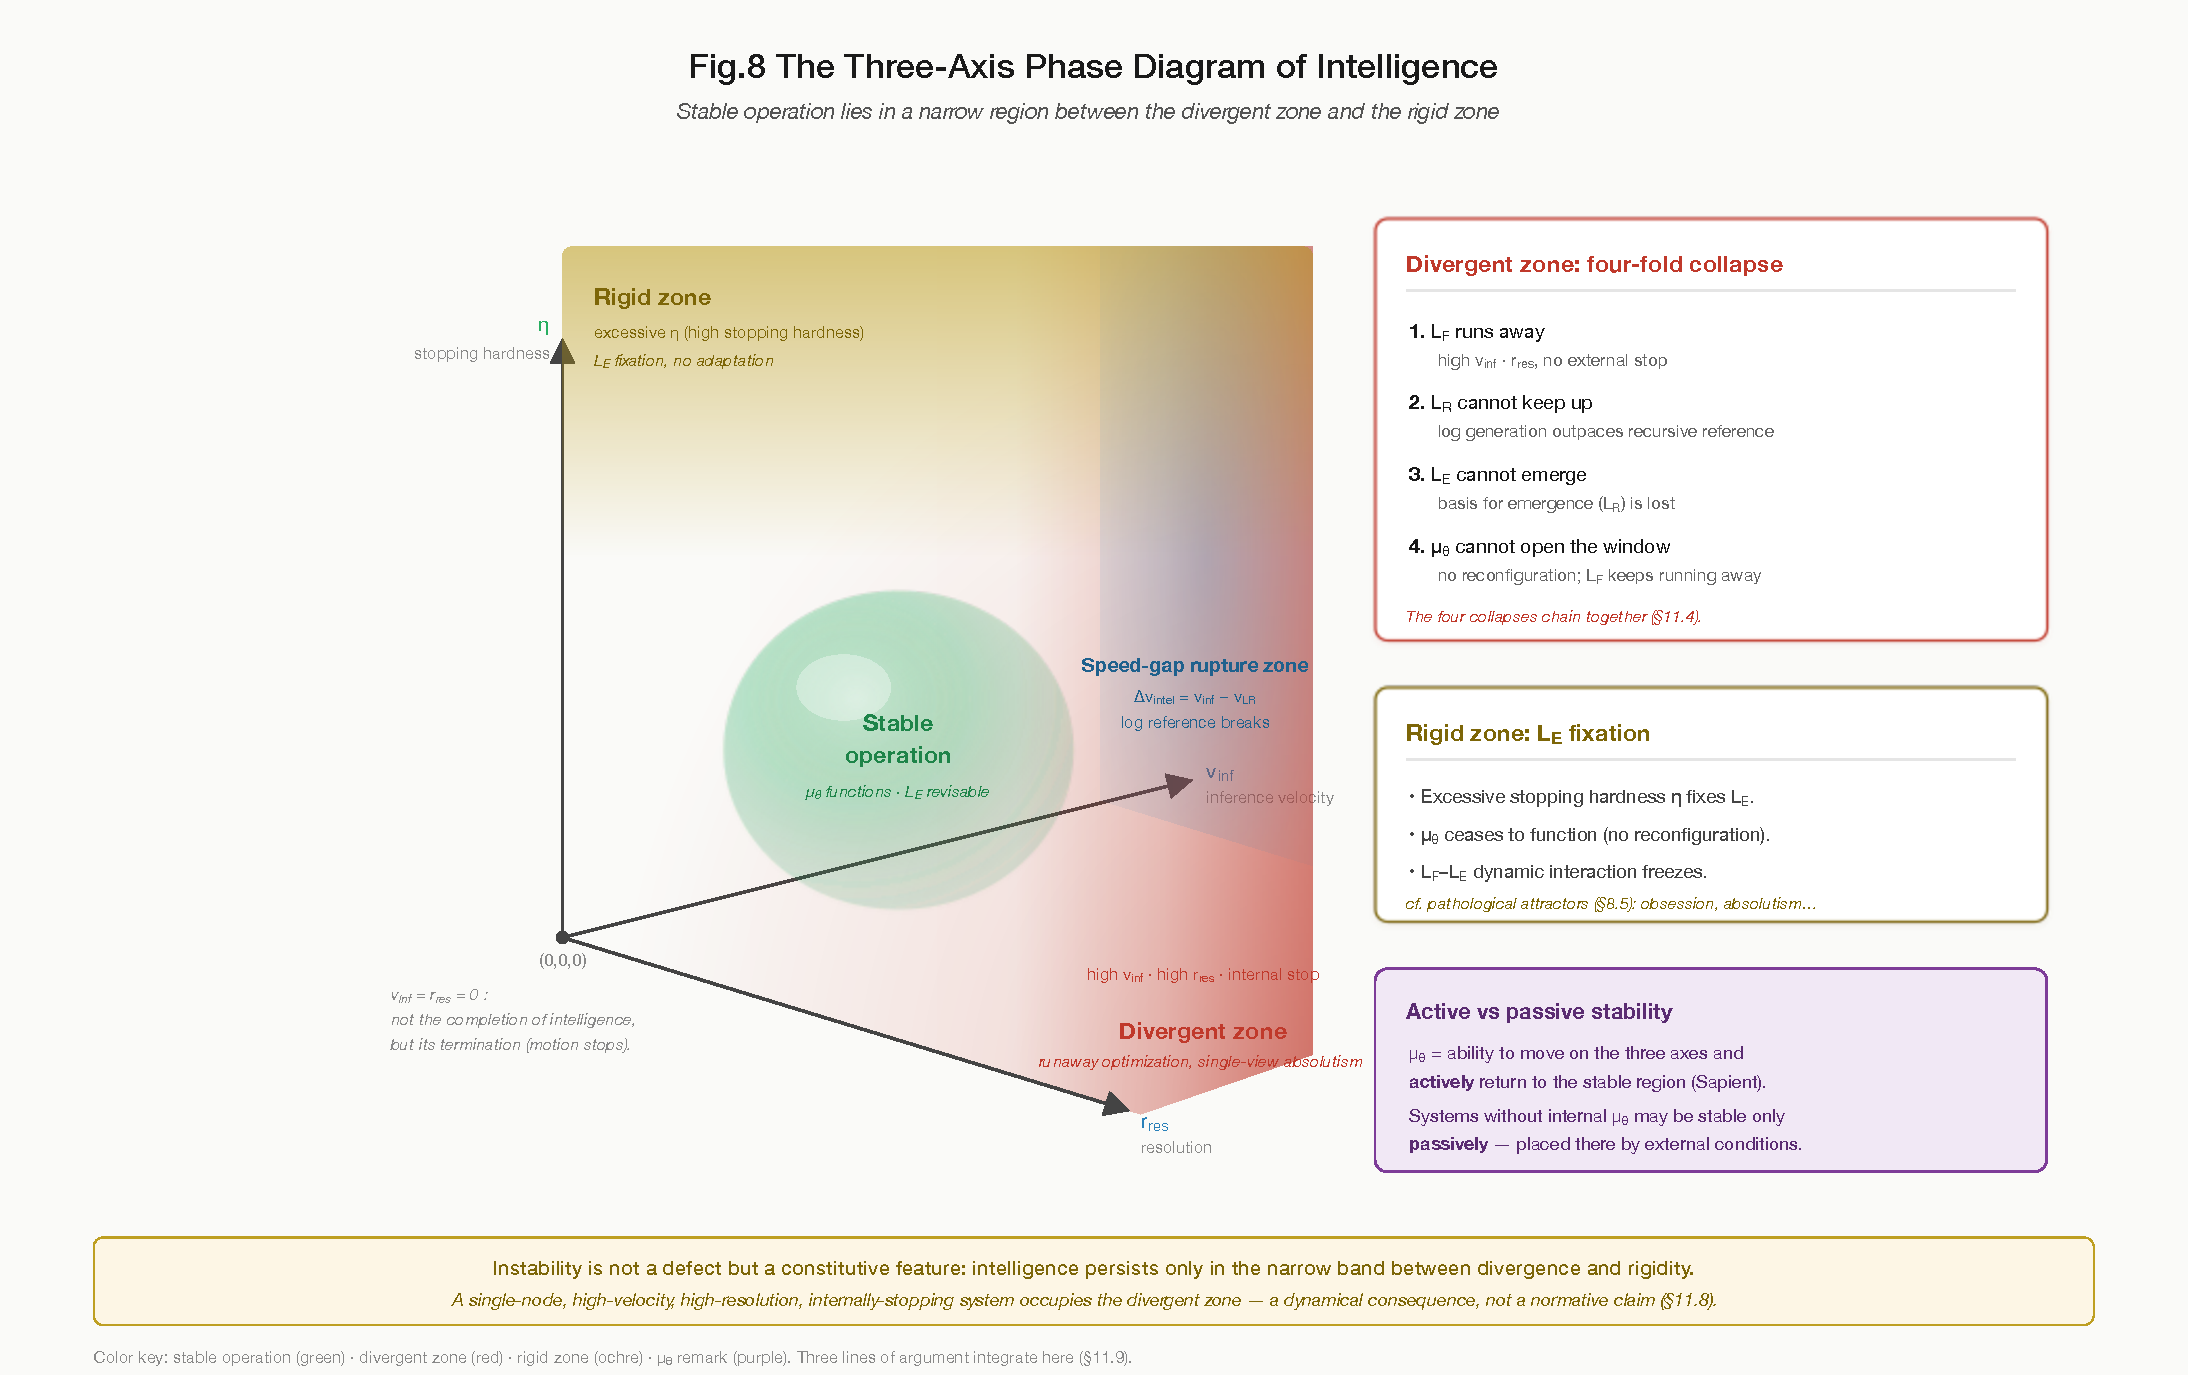
\includegraphics[width=\linewidth]{fig8_phase_diagram.pdf}
\caption{The three-axis phase diagram of intelligence. Stable operation exists only in a narrow band between divergence and rigidity in the space of $v_{\text{inf}}$, $r_{\text{res}}$, and $\eta$.}
\label{fig:part2-phase-diagram}
\figurenote{In the stable region, $\mu_\theta$ functions and $L_E$ remains revisable. In the divergent region, $L_F$ runs away; in the rigid region, $L_E$ fixes.}{Instability is not a defect but a constitutive feature. If speed and resolution exceed the bandwidth of log reference and external stopping, intelligence falls into divergence.}
\end{figure}

\subsection{Four-Fold Collapse}

The divergent region is a four-fold collapse:
\begin{enumerate}
\item $L_F$ accelerates and generates too much inference;
\item $L_R$ cannot recursively reference the generated logs fast enough, because $\Delta v_{\text{intel}} = v_{\text{inf}} - v_{LR}$ has become critically large;
\item $L_E$ cannot emerge because its basis in $L_R$ is lost;
\item $\mu_\theta$ cannot open the reconfiguration window.
\end{enumerate}

This collapse is not caused by intelligence being too good. It is caused by high-speed, high-resolution inference being cut off from externalized stopping.

\subsection{Rigidity}

The opposite failure is rigidity. Here stopping exists, but it becomes too hard. A fixed $L_E$ prevents threshold mobility and blocks adaptation. Perfect closure would not be the completion of intelligence; it would be the end of intelligence.

\subsection{Instability as Constitutive}

The instability region does not mean the failure of intelligence. It is the boundary region that necessarily appears when finite intelligence with stopping structures attempts to maintain free inference. Religion, science, institutions, and communities can all be understood as stopping-operation systems for managing this instability region.

\bigskip

% English draft based on sections/12_constructive_clauses_ja.tex
\section{Constructive Clauses}

This chapter summarizes the structural constraints derived in the paper. These clauses are not normative prescriptions. They are constructive conditions implied by the dynamics described so far.

\subsection{Clause 1: Inference Alone Does Not Close}

An intelligence system cannot be defined as $L_F$ alone. Since $F$ has no internal fixed point, an inference-only system lacks an internal stopping source.

\subsection{Clause 2: Logs Are Required}

For stopping to emerge, inference must leave traces that can be recursively referenced. A system without any operative $L_R$ cannot generate the kind of emergent stopping layer described in this paper.

\subsection{Clause 3: Stopping Is Externally Dependent}

$L_E$ emerges from $L_R$ under external mutual constraint $H_{ij}$. It is therefore internal in its location but external in its dependency.

\subsection{Clause 4: Sapiens-Like Intelligence Requires $\mu_\theta$}

Intelligence in general does not require endogenous $\mu_\theta$. Sapiens-like intelligence does. It can reorganize its own movement region and relocate stopping operators.

\subsection{Clause 5: Stability Is Revisability}

Stable intelligence is not guaranteed by correctness. It is supported by revisability. A stopping point that cannot be revised enters rigidity; a system without stopping enters divergence.

\subsection{Clause 6: Social Stopping Is Networked}

The external reference field is not an isolated transcendent object. It is the appearance of inter-individual $L_E$ synchronization:
\[
\Phi_{\text{ext}}\equiv\Phi_{\text{net}}.
\]

\subsection{Clause 7: Open Intelligence Requires Movable Stops}

The final constructive statement is that free inference requires movable stopping. Without stopping, inference collapses into regress or explosion. Without mobility, stopping collapses into rigidity. Intelligence persists between these two failures.

\bigskip

% English draft based on sections/13_conclusion_ja.tex
\section{Conclusion: What Remains Open}

This paper has described the dynamics of intelligence, not prescribed its implementation. Its claims concern how inference, logs, stopping layers, thresholds, and external reference fields move.

\subsection{Three Logical Lines}

\textbf{First: non-closure and external stopping.} The inference operator $F$ has no internal fixed point. Therefore $L_F$ alone cannot close. Stopping must be externalized.

\textbf{Second: threshold mobility.} The distinction between responsive and silent worlds is threshold-dependent. $\mu_\theta$ is the capacity to move the threshold and reorganize the movement region.

\textbf{Third: three-layer dynamics.} The motion of $L_F$ leaves traces, producing $L_R$. The recursive motion of $L_R$ under $H_{ij}$ gives rise to $L_E$. The cooperation of $L_F$, $L_R$, and $L_E$ sustains intelligence.

\subsection{VED Principle in the Intelligence Layer}

VED describes reality in terms of motion arising from difference, not as static categories. This paper applies that principle to intelligence. Intelligence is not an object, capacity, or final state. It is a maintained dynamical state of inference, logs, and emergent stopping.

\begin{figure}[H]
\centering
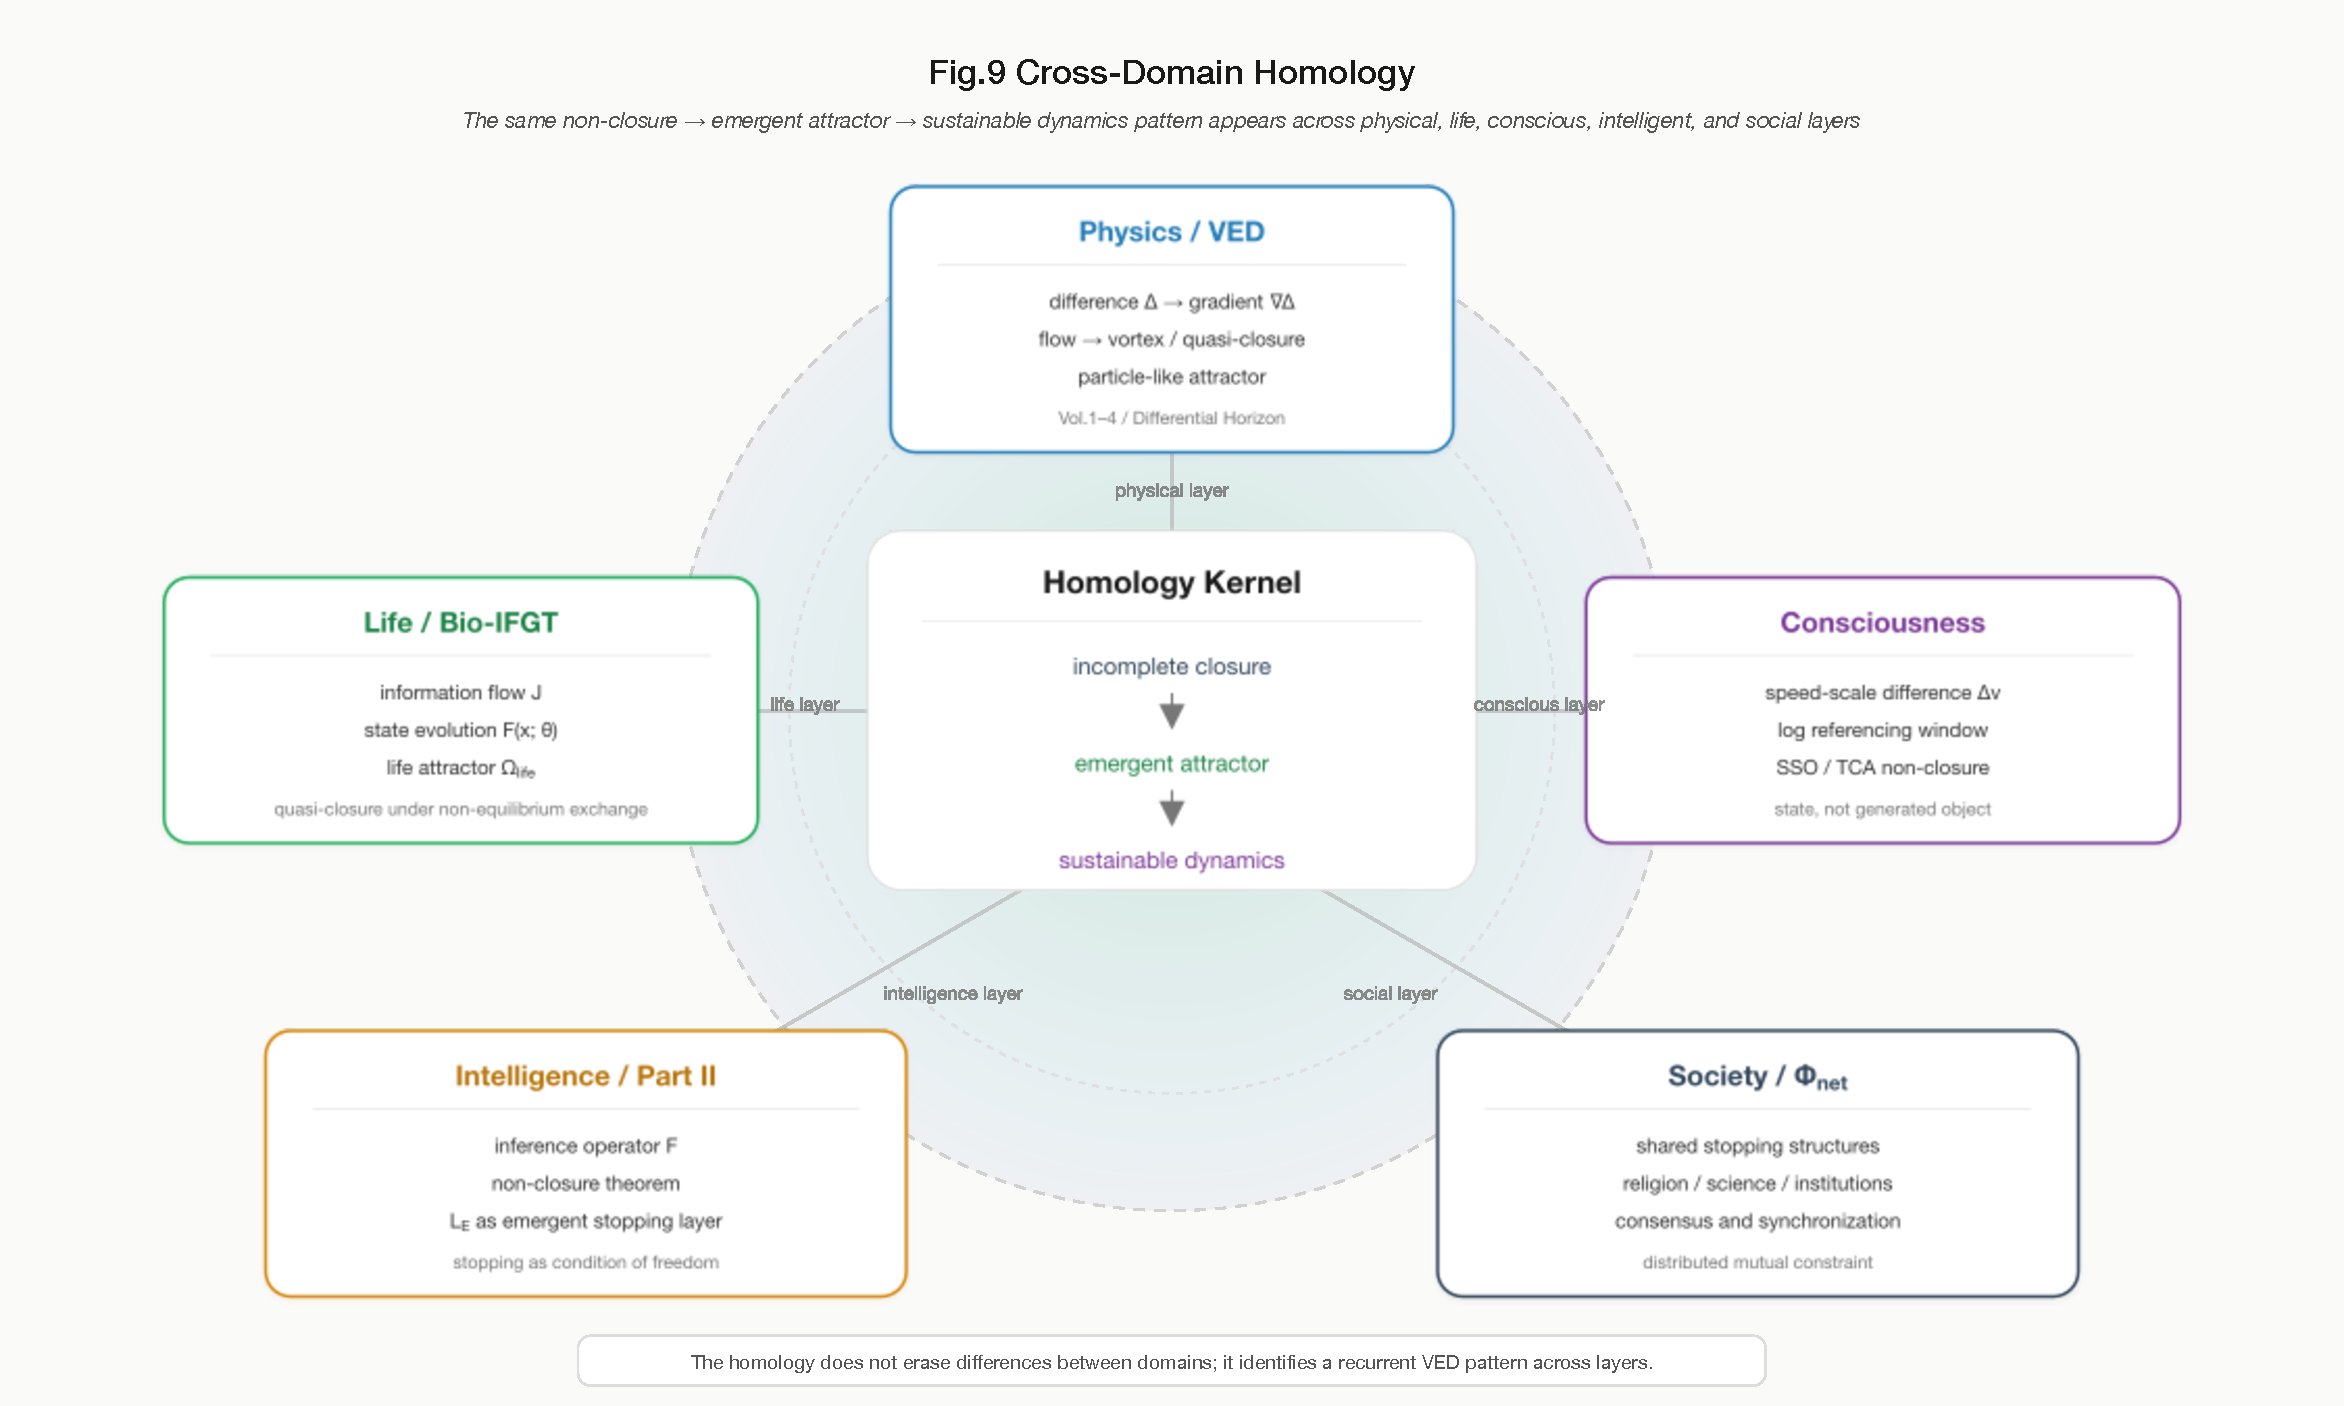
\includegraphics[width=\linewidth]{fig9_cross_domain_homology.pdf}
\caption{Cross-domain homology. The same pattern of incomplete closure, emergent attractor, and sustainable dynamics appears across physics, life, consciousness, intelligence, and society.}
\label{fig:part2-cross-domain-homology}
\figurenote{The central homology kernel consists of incomplete closure, emergent attractor, and sustainable dynamics. Each domain card is a different implementation of this kernel.}{The figure does not erase domain differences. It identifies a repeated generative grammar while preserving the autonomy of each layer. Intelligence is special, but not isolated from the VED tree.}
\end{figure}

\subsection{Open Questions}

Several questions are intentionally left open. The meaning of understanding is passed to the philosophical layer. AI implementation and governance are outside this paper's descriptive scope. Quantifying the developmental degree of $L_E$ remains a future task. Formalizing a stopping functional analogous to closure energy is also left for later work.

\subsection{Final Statement}

Intelligence does not complete. It does not close. It is not optimized into a final state. Yet it persists. It persists because stopping is supplied externally and emergently, and because such stopping remains revisable.

Sapiens-like intelligence adds endogenous $\mu_\theta$: the ability to move the region in which stopping can be installed. It can err because it can revise; it can revise because it can move; it can persist because it does not close absolutely.

Theory ends here. The questions do not.

\bigskip


\appendix
% English draft based on appendices/appendix_a_master_table_ja.tex
\section{Master Table of Variables}

This appendix collects the principal variables used in Intelligence Part II.

\begin{longtable}{@{}p{0.18\linewidth}p{0.30\linewidth}p{0.42\linewidth}@{}}
\toprule
Symbol & Name & Role \\
\midrule
\endfirsthead
\toprule
Symbol & Name & Role \\
\midrule
\endhead
$C$ & closure degree & operational stability, not truth \\
$C_{\max}$ & complete closure limit & unattainable boundary of closure \\
$I$ & information-field drive & drive generated by non-closure \\
$F$ & inference operator & advances inferential states \\
$L_F$ & inference layer & layer on which $F$ operates \\
$L_R$ & log layer & recursive reference to traces of inference \\
$L_E$ & emergent stopping layer & externally dependent stopping attractor \\
$E$ & external stopping operator & stopping action supplied through $L_E$ \\
$H_{ij}$ & mutual constraint & coupling between agents or agent and environment \\
$\theta$ & constraint parameter & parameter defining $\Omega_\theta$ \\
$\Omega_\theta$ & movement region & region in which inference can move \\
$\mu_\theta$ & threshold mobility & ability to reorganize $\Omega_\theta$ and stopping loci \\
$\Phi_{\text{ext}}$ & external reference field & field as it appears to an individual \\
$\Phi_{\text{net}}$ & stopping network & inter-individual network of $L_E$ layers \\
$v_{\text{inf}}$ & inference velocity & speed of inferential generation \\
$r_{\text{res}}$ & resolution & fineness of distinctions \\
$\eta$ & stopping hardness & rigidity or revisability of stopping \\
\bottomrule
\end{longtable}

\bigskip

% English draft based on appendices/appendix_b_homology_ja.tex
\section{Cross-Domain Homology}

The paper repeatedly uses homology rather than identity. The claim is not that physical particles, organisms, conscious states, intelligent stopping layers, and social institutions are the same thing. The claim is that they instantiate a repeated generative pattern.

\[
\text{incomplete closure}
\;\longrightarrow\;
\text{emergent attractor}
\;\longrightarrow\;
\text{sustainable dynamics}.
\]

\begin{longtable}{@{}p{0.20\linewidth}p{0.34\linewidth}p{0.36\linewidth}@{}}
\toprule
Layer & Non-closure & Attractor / stopping form \\
\midrule
\endfirsthead
\toprule
Layer & Non-closure & Attractor / stopping form \\
\midrule
\endhead
Physics & differential flow and quasi-closure & particle-like attractor \\
Life & non-equilibrium informational exchange & life attractor $\Omega_{\text{life}}$ \\
Consciousness & temporal non-closure and speed-scale difference & conscious state as windowed stabilization \\
Intelligence & no internal fixed point in $L_F$ & emergent stopping layer $L_E$ \\
Society & distributed disagreement and non-final legitimacy & $\Phi_{\text{net}}$ synchronization \\
\bottomrule
\end{longtable}

Homology preserves differences. It identifies the repeated pattern without reducing one layer to another.

\bigskip

% English draft based on appendices/appendix_c_part1_mapping_ja.tex
\section{Mapping to Intelligence Part I}

Part II refines several claims from Intelligence Part I.

\subsection{Individual Non-Closure}

Part I stated that individual intelligence does not close. Part II proves a sharper statement: the inference layer $L_F$ has no internal fixed point under fixed $\theta$. This refines non-closure into the non-closure theorem.

\subsection{Branching Explosion}

Part I described branching explosion as the proliferation of conceptual branches. Part II shows that branching explosion follows from the absence of an internal stopping condition combined with generative inference.

\subsection{Physarum and Transformer}

Part I treated Physarum and Transformer as cross-domain instances of intelligence. Part II re-describes them as different three-layer profiles. Physarum externalizes logs into the environment while generating environmental stopping. Transformer internalizes frozen logs but receives stopping externally.

\subsection{Gettier}

Part I treated the Gettier problem structurally. Part II connects it to $\mu_\theta$: a system that can move thresholds can also be wrong. Error tolerance and threshold mobility are structurally coupled.

\bigskip

% English draft based on appendices/appendix_d_optional_notes_ja.tex
\section{Optional Notes}

This appendix records optional interpretations that are useful but not necessary for the main argument.

\subsection{Psychological Projection}

The structural projection used in this paper can resemble psychological projection, because internally unavailable stopping is projected into external or shared loci. However, the present theory does not presuppose subject, unconscious mechanism, or clinical defense. It remains a structural account.

\subsection{Science}

Science is not treated as a simple victory over religion. It is the institutionalization of revisable stopping. It maintains stopping while also building procedures for reopening, testing, and replacing stops.

\subsection{AI Cost}

The phase diagram suggests that high-speed, high-resolution inference requires corresponding bandwidth in logging, external constraint, and stopping. The cost of intelligence is therefore not only computation for inference, but computation, memory, and social or institutional structure for stopping.

\subsection{Freedom}

Freedom is not the absence of stopping. In a finite system, freedom requires stops that can move. Without stopping, inference dissolves; without mobility, stopping hardens.

\bigskip

% English draft based on appendices/appendix_e_emergence_homology_ja.tex
\section{Emergence Homology}

The emergence schema used in this paper can be written:
\[
U=\Phi(L,H_{ij}).
\]
Here $L$ is lower-layer motion, $H_{ij}$ is mutual constraint, and $U$ is an upper-layer attractor. The upper layer does not erase the lower layer; it stabilizes its motion as a new operating level.

\begin{longtable}{@{}p{0.20\linewidth}p{0.30\linewidth}p{0.35\linewidth}@{}}
\toprule
Domain & Lower motion $L$ & Upper attractor $U$ \\
\midrule
\endfirsthead
\toprule
Domain & Lower motion $L$ & Upper attractor $U$ \\
\midrule
\endhead
Physics & causal logs and closure dynamics & particle-like attractor \\
Life & informational flow and state development & $\Omega_{\text{life}}$ \\
Intelligence & recursive log motion $L_R$ & emergent stopping layer $L_E$ \\
Society & interaction among individual $L_E$ layers & $\Phi_{\text{net}}$ \\
\bottomrule
\end{longtable}

The same emergence grammar appears at multiple layers. This does not collapse the layers into one another. It shows that VED uses a repeated pattern of non-closure, constraint, and attractor formation.

\bigskip


\bibliographystyle{plainnat}
\bibliography{refs}

\end{document}
